% ============================================================
%  Diplomingeniørprojekt – DTU Software Technology
%  Kompiler med: pdfLaTeX (Overleaf standard)
% ============================================================
\documentclass[12pt, a4paper, oneside]{report}

% ── Encoding & sprog ────────────────────────────────────────
\usepackage[utf8]{inputenc}
\usepackage[T1]{fontenc}
\usepackage[danish]{babel}

% ── Skrifttype ───────────────────────────────────────────────
\usepackage{lmodern}
\usepackage{microtype}           % Bedre orddeling og spacing
\emergencystretch=3em
% ── Sidelayout ───────────────────────────────────────────────
\usepackage[
  a4paper,
  top=3cm, bottom=3cm,
  left=2.8cm, right=2.8cm
]{geometry}
\usepackage{setspace}
\setstretch{1.2}
\setlength{\parskip}{6pt}
\setlength{\parindent}{0pt}


% ── Farver ───────────────────────────────────────────────────
\usepackage[dvipsnames]{xcolor}
\definecolor{dtuRed}{RGB}{153,0,0}
\definecolor{arkynBlue}{RGB}{29,130,219}
\definecolor{codeBackground}{RGB}{248,248,248}
\definecolor{codeComment}{RGB}{106,153,85}
\definecolor{codeKeyword}{RGB}{86,156,214}
\definecolor{codeString}{RGB}{206,145,120}
\definecolor{codeType}{RGB}{78,201,176}
\definecolor{codePurple}{RGB}{197,134,192}

% ── Figurer & tabeller ───────────────────────────────────────
\usepackage{graphicx}
\usepackage{float}
\usepackage{booktabs}
\usepackage{tabularx}
\usepackage{array}
\usepackage{multirow}
\usepackage{caption}
\usepackage{subcaption}
\captionsetup{font=small, labelfont=bf, skip=6pt}

% ── Kodelistings ─────────────────────────────────────────────
\usepackage{listings}

% Grundlæggende stil
\lstdefinestyle{base}{
  backgroundcolor=\color{codeBackground},
  basicstyle=\ttfamily\small,
  breakatwhitespace=false,
  breaklines=true,
  captionpos=b,
  commentstyle=\color{codeComment}\itshape,
  frame=single,
  framesep=4pt,
  framerule=0.5pt,
  rulecolor=\color{gray!30},
  keepspaces=true,
  keywordstyle=\color{codeKeyword}\bfseries,
  numbers=left,
  numbersep=8pt,
  numberstyle=\tiny\color{gray},
  showspaces=false,
  showstringspaces=false,
  showtabs=false,
  stringstyle=\color{codeString},
  tabsize=4,
  xleftmargin=1.5em,
}

% Swift
\lstdefinelanguage{Swift}{
  morekeywords={
    func,var,let,class,struct,enum,protocol,extension,import,
    return,if,else,guard,switch,case,default,for,while,do,try,
    catch,throw,throws,async,await,actor,nil,true,false,self,
    super,init,deinit,get,set,willSet,didSet,lazy,static,final,
    override,open,public,internal,private,fileprivate,mutating,
    nonmutating,in,where,as,is,some,any,@MainActor,@Published,
    @StateObject,@ObservedObject,@State,@Binding,@AppStorage,
    @EnvironmentObject,@Environment,ObservableObject,View,
    Task,MainActor
  },
  morestring=[b]",
  morestring=[b]""",
  morecomment=[l]{//},
  morecomment=[s]{/*}{*/},
  sensitive=true
}

% Go
\lstdefinelanguage{Go}{
  morekeywords={
    break,case,chan,const,continue,default,defer,else,fallthrough,
    for,func,go,goto,if,import,interface,map,package,range,return,
    select,struct,switch,type,var,nil,true,false,error,
    string,int,int64,float64,bool,byte,rune,uint,uint64
  },
  morestring=[b]",
  morestring=[b]`,
  morecomment=[l]{//},
  morecomment=[s]{/*}{*/},
  sensitive=true
}

\lstset{style=base,
  literate=
    {ø}{{\o}}1 {æ}{{\ae}}1 {å}{{\aa}}1
    {Ø}{{\O}}1 {Æ}{{\AE}}1 {Å}{{\AA}}1
}

% Shorthand kommandoer til sprog
\newcommand{\swift}[1]{\lstinline[language=Swift]{#1}}
\newcommand{\gocode}[1]{\lstinline[language=Go]{#1}}

% ── Matematik ────────────────────────────────────────────────
\usepackage{amsmath}
\usepackage{amssymb}

% ── Citater ──────────────────────────────────────────────────
\usepackage[danish=guillemets]{csquotes}

% ── Referencer (IEEE-stil) ───────────────────────────────────
\usepackage[
  backend=biber,
  style=ieee,
  sorting=none
]{biblatex}
\addbibresource{references.bib}

% ── Sidehoved og -fod ────────────────────────────────────────
\usepackage{fancyhdr}
\pagestyle{fancy}
\fancyhf{}
\renewcommand{\headrulewidth}{0.4pt}
\fancyhead[L]{\small\leftmark}
\fancyhead[R]{\small\thepage}
\fancypagestyle{plain}{
  \fancyhf{}
  \renewcommand{\headrulewidth}{0pt}
  \fancyfoot[C]{\small\thepage}
}

% ── Kapitelformatering ───────────────────────────────────────
\usepackage{titlesec}
\titleformat{\chapter}[hang]
  {\normalfont\LARGE\bfseries\color{dtuRed}}
  {\thechapter}{1em}{}
\titlespacing{\chapter}{0pt}{0pt}{20pt}

\titleformat{\section}
  {\normalfont\Large\bfseries}
  {\thesection}{1em}{}

\titleformat{\subsection}
  {\normalfont\large\bfseries}
  {\thesubsection}{1em}{}

% ── Hyperlinks ───────────────────────────────────────────────
\usepackage[
  colorlinks=true,
  linkcolor=dtuRed,
  citecolor=arkynBlue,
  urlcolor=arkynBlue,
  pdftitle={OCR- og AI-baseret maskinidentifikation},
  pdfauthor={Peter Hannibal Hildorf}
]{hyperref}

% ── Nyttige pakker ───────────────────────────────────────────
\usepackage{enumitem}
\usepackage{pifont}
\usepackage{mdframed}          % Til info-bokse
\usepackage{tcolorbox}         % Til farvede bokse
\tcbuselibrary{most}

% Definér en "info-boks"
\newtcolorbox{infobox}[1][]{
  colback=arkynBlue!8,
  colframe=arkynBlue!60,
  fonttitle=\bfseries,
  title=#1,
  left=6pt, right=6pt, top=4pt, bottom=4pt
}

% Definér en "advarselsboks"
\newtcolorbox{warningbox}[1][]{
  colback=orange!8,
  colframe=orange!60,
  fonttitle=\bfseries,
  title=#1,
  left=6pt, right=6pt, top=4pt, bottom=4pt
}

% ============================================================
%  DOKUMENT
% ============================================================
\begin{document}

% ── Titelside ────────────────────────────────────────────────
\begin{titlepage}
  \centering
  
\includegraphics[width=4cm]{figures/dtu_logo}

  \vspace*{1.5cm}

  {\large\textbf{DTU Software Technology}}\\[0.3cm]
  {\normalsize Department of Engineering Technology and Didactics}\\[0.2cm]
  {\normalsize Diplomingeniørprojekt}\\[0.5cm]

  \noindent\rule{\textwidth}{1pt}\\[0.6cm]

  {\LARGE\bfseries OCR- og AI-baseret maskinidentifikation\\[0.3cm]
  til vedligeholdelsesteknikere}\\[0.4cm]
  {\large En mobil prototype til Arkyn Studios}

  \\[0.4cm]\noindent\rule{\textwidth}{1pt}

  \vspace{2.5cm}

  \begin{minipage}{0.45\textwidth}
    \centering

    \textbf{FORFATTER}\\[0.3cm]
    Peter Hannibal Hildorf\\
    \texttt{s[studienummer]}
  \end{minipage}
  \hfill
  \begin{minipage}{0.45\textwidth}
    \centering
    \textbf{VEJLEDER}\\[0.3cm]
    [Vejledernavn]\\
    DTU
  \end{minipage}

  \vspace{2.5cm}

  {\normalsize Maj 2026}

  \vfill

  % Indsæt DTU-logo: gem dtu_logo.png i figures/ og fjern %-tegnet nedenfor

  \vspace{1cm}
\end{titlepage}

% ── Forord (valgfrit) ────────────────────────────────────────
% Fjern kommentering hvis du vil tilføje forord
% \chapter*{Forord}
% \addcontentsline{toc}{chapter}{Forord}
% Tekst her...
% \clearpage

% ── Abstract ─────────────────────────────────────────────────
\chapter*{Abstract}
\addcontentsline{toc}{chapter}{Abstract}
\thispagestyle{plain}

% TODO: Skriv abstract sidst – efter alle andre kapitler er færdige.
% Ca. 200–250 ord på engelsk. Eksempel på struktur:
%
% This project presents the development of a mobile prototype feature for
% maintenance technicians at Arkyn Studios. The system enables rapid machine
% identification through image- and video-based Optical Character Recognition
% (OCR), followed by AI-generated maintenance guidance. [...]

\textit{(Skrives sidst — se kommentar i main.tex)}

\clearpage

% ── Indholdsfortegnelse ──────────────────────────────────────
\tableofcontents
\clearpage

% ── Figurliste (tilføj hvis du har mange figurer) ────────────
% \listoffigures
% \addcontentsline{toc}{chapter}{Figurliste}
% \clearpage

% ── Kapitelindhold ───────────────────────────────────────────
x\chapter{Introduktion}
\label{chap:introduction}

\section{Baggrund}
\label{sec:baggrund}

Arkyn Studios er en dansk softwarevirksomhed, der udvikler digitale løsninger til enterprise-virksomheder med fokus på vedligeholdelse af maskiner og udstyr i produktionsmiljøer. Virksomhedens kerneprodukt er en mobil applikation, der understøtter teknikernes daglige arbejde på fabriksgulvet — fra registrering af opgaver til dokumentation af udført vedligehold.

I takt med at produktionsmiljøer automatiseres og specialiseres, oplever mange virksomheder et stigende behov for digital støtte til de medarbejdere, der udfører vedligeholdelsesopgaverne i praksis. Arkyn Studios' kunder har specifikt givet udtryk for, at fremtidens vedligeholdelsesteknikere i stigende grad vil have en mere generalistisk baggrund, og dermed have mindre dybdegående kendskab til den specifikke maskinpark de arbejder med. Dette stiller nye krav til de digitale værktøjer, der skal støtte dem i arbejdet.

Dette projekt er gennemført i tilknytning til et praktikophold hos Arkyn Studios og tager udgangspunkt i en konkret problemstilling identificeret i samarbejde med virksomheden.

\section{Problemformulering}
\label{sec:problemformulering}

En konkret og gentagen udfordring i vedligeholdelsesarbejdet er, at teknikeren hurtigt skal kunne identificere en maskine og finde relevant information om dens vedligeholdelse — særligt i situationer, hvor maskinen ikke er umiddelbart genkendelig, eller hvor teknikeren ikke har erfaring med netop denne maskintype.

I dag sker denne identifikation primært manuelt: teknikeren aflæser maskinens typeskilt eller mærkat og søger derefter i dokumentation eller kontakter en mere erfaren kollega. Denne proces er tidskrævende, fejlbehæftet og afhænger i høj grad af den individuelle teknikers erfaring og viden.

Selvom teknologier som Optical Character Recognition (OCR) og kunstig intelligens eksisterer som separate løsninger, er integrationen af billedbaseret input og AI-assisteret vejledning i en vedligeholdelseskontekst fortsat et åbent og relevant problemfelt.

\begin{infobox}[Problemformulering]
Hvordan kan en mobilapplikation ved hjælp af OCR og AI-genereret vejledning understøtte vedligeholdelsesteknikere i hurtig identifikation af maskiner og adgang til relevant vedligeholdelsesinformation?
\end{infobox}

\section{Projektmål}
\label{sec:projektmaal}

På baggrund af problemformuleringen er følgende konkrete mål fastsat for projektet:

\begin{enumerate}
  \item Udvikle en prototype på en mobil feature til iOS, der muliggør billedbaseret identifikation af maskiner ved optagelse af typeskilte og maskinlabels
  \item Implementere en pipeline der via OCR udtrækker struktureret information fra billeder og korte videoer
  \item Integrere en AI-baseret service, der på baggrund af den udtrukne information genererer forståelig og handlingsorienteret vedligeholdelsesvejledning
  \item Designe et simpelt og effektivt brugerflow baseret på etablerede usability-principper, der fungerer i en industriel arbejdskontekst
  \item Evaluere systemets tekniske funktionalitet og brugbarhed i samarbejde med Arkyn Studios
\end{enumerate}

\section{Afgrænsning}
\label{sec:afgrænsning}

Projektet er afgrænset til udviklingen af en prototype, og følgende er bevidst udeladt af scope:

\textbf{Ingen ERP/SAP-integration:} Systemet henter ikke information fra virksomhedsspecifikke systemer. Al vejledning genereres på baggrund af generel industriel viden fra AI-modellen.

\textbf{iOS only:} Applikationen er udelukkende udviklet til iOS (iPhone og iPad) og understøtter ikke Android i den nuværende prototype.

\textbf{Ingen autentificering:} Prototypen implementerer ikke brugerlogin eller rollestyring, da fokus er på kerneflowet frem for sikkerhedsinfrastruktur.

\textbf{Begrænset maskindomæne:} Systemet er ikke specialiseret til én bestemt maskintype, men demonstreres med generelle industrielle maskiner og udstyr.


\chapter{Analyse og kravspecifikation}
\label{chap:analysis}

\section{Domæneanalyse}
\label{sec:domæneanalyse}

For at forstå det problem systemet skal løse, er det nødvendigt at analysere den kontekst, hvori vedligeholdelsesteknikeren arbejder. Denne analyse tager udgangspunkt i information indsamlet i samarbejde med Arkyn Studios samt de erfaringer der er gjort i løbet af praktikopholdet.

\subsection{Teknikerens arbejdssituation}
\label{subsec:teknikerens-arbejdssituation}

En vedligeholdelsesteknikers arbejdsdag er præget af uforudsigelige hændelser: maskiner der går ned, fejl der skal diagnosticeres og udstyr der skal inspiceres. Arbejdet foregår på fabriksgulvet — typisk under tidspres, i støjende omgivelser og med begrænset adgang til stationære computere og dokumentation.

Når en teknikeren møder en ukendt maskine eller et ukendt udstyr, følger typisk dette forløb:

\begin{enumerate}
  \item \textbf{Identifikation:} Teknikeren forsøger at identificere maskinen ved at aflæse typeskilt, mærkat eller stregkode — hvis disse overhovedet er læselige efter års slitage og industrielt miljø.
  \item \textbf{Informationssøgning:} På baggrund af den identificerede model eller serienummer søges i virksomhedens dokumentationssystem, papirmanualer eller via kolleger.
  \item \textbf{Udførelse:} Teknikeren udfører vedligeholdelsen baseret på fundet information — eller på bedste skøn, hvis informationen er utilstrækkelig.
\end{enumerate}

Dette forløb er forbundet med kendte smertepunkter: typeskilte kan være ulæselige eller på fremmedsprog, dokumentation kan være svær at finde, og afhængighed af erfarne kolleger skaber flaskehalse i organisationen.

\subsection{Teknologisk kontekst}
\label{subsec:teknologisk-kontekst}

Centrale teknologier i løsningsrummet er:

\textbf{Optical Character Recognition (OCR):} Teknologi til automatisk tekstgenkendelse i billeder. I industriel kontekst anvendes OCR til aflæsning af typebetegnelser, serienumre og tekniske specifikationer fra maskinlabels. Moderne cloud-baserede OCR-løsninger som Google Cloud Vision~\cite{google_vision} opnår høj nøjagtighed selv på skæve vinkler og delvist slidte labels.

\textbf{Large Language Models (LLM):} AI-modeller der kan fortolke struktureret tekstinformation og generere handlingsorienterede vejledninger på naturligt sprog. Modeller som Anthropic Claude~\cite{anthropic_claude} kan instrueres til at returnere struktureret JSON-output, hvilket letter integration med eksisterende systemer.

\textbf{Mobilkamera:} Moderne smartphones har kameraer af tilstrækkelig kvalitet til at fungere som input-enhed for OCR-behandling, og giver teknikeren et allerede velkendt og tilgængeligt redskab.

Selvom de individuelle teknologier er velkendte, er kombinationen af billedbaseret input, realtids-OCR og AI-assisteret vejledning i en vedligeholdelseskontekst et relativt uudforsket område.

\section{Brugsscenarier}
\label{sec:brugsscenarier}

På baggrund af domæneanalysen er følgende primære brugsscenarier identificeret.

\subsection{Use Case 1: Billede af typeskilt}

\begin{tabular}{@{}lp{0.7\textwidth}@{}}
  \toprule
  \textbf{Aktør}        & Vedligeholdelsesteknikeren \\
  \textbf{Forudsætning} & Teknikeren er i nærheden af en maskine med et synligt typeskilt \\
  \midrule
  \multicolumn{2}{@{}l@{}}{\textbf{Forløb}} \\
  1 & Teknikeren åbner applikationen og navigerer til kamera-fanen \\
  2 & Der tages et billede af maskinens typeskilt \\
  3 & Systemet kører OCR og returnerer strukturerede entiteter (producent, model, serienummer mv.) \\
  4 & Teknikeren trykker \textit{Analyser} på den ønskede entitet \\
  5 & Systemet returnerer AI-genereret vedligeholdelsesvejledning \\
  \midrule
  \textbf{Resultat} & Teknikeren modtager relevant information inden for få sekunder \\
  \bottomrule
\end{tabular}

\vspace{1em}

\subsection{Use Case 2: Video af stor label}

\begin{tabular}{@{}lp{0.7\textwidth}@{}}
  \toprule
  \textbf{Aktør}        & Vedligeholdelsesteknikeren \\
  \textbf{Forudsætning} & Maskinens label er for stor til at blive fotograferet i ét billede \\
  \midrule
  \multicolumn{2}{@{}l@{}}{\textbf{Forløb}} \\
  1 & Teknikeren optager en kort video ved at panorere kameraet henover labelen \\
  2 & Systemet behandler videoen ved at udtrække frames (1 FPS) og køre OCR på hver enkelt \\
  3 & Systemet aggregerer den udtrukne tekst og returnerer strukturerede entiteter \\
  4--5 & Som Use Case 1, trin 4--5 \\
  \midrule
  \textbf{Resultat} & Komplet tekstudtræk fra labels der er for store til ét billede \\
  \bottomrule
\end{tabular}

\vspace{1em}

\subsection{Use Case 3: Lav billedkvalitet}

\begin{tabular}{@{}lp{0.7\textwidth}@{}}
  \toprule
  \textbf{Aktør}        & Vedligeholdelsesteknikeren \\
  \textbf{Forudsætning} & Billede er optaget under dårlige lysforhold, eller typeskiltet er snavset \\
  \midrule
  \multicolumn{2}{@{}l@{}}{\textbf{Forløb}} \\
  1 & Teknikeren uploader et billede som normalt \\
  2 & Systemet registrerer lav OCR-confidence (under 60~\%) \\
  3 & Systemet markerer resultatet som \textit{Manuel kontrol påkrævet} \\
  4 & Teknikeren informeres om at tage et nyt, tydeligere billede \\
  \midrule
  \textbf{Resultat} & Systemet fejler kontrolleret frem for at returnere forkerte data \\
  \bottomrule
\end{tabular}

\section{Kravspecifikation}
\label{sec:krav}

\subsection{Funktionelle krav}
\label{subsec:funktionelle-krav}

Tabel~\ref{tab:funktionelle-krav} opstiller de funktionelle krav til systemet, udledt fra domæneanalysen og brugsscenariet.

\begin{table}[H]
  \centering
  \caption{Funktionelle krav}
  \label{tab:funktionelle-krav}
  \begin{tabularx}{\textwidth}{@{}llX@{}}
    \toprule
    \textbf{ID} & \textbf{Krav} & \textbf{Beskrivelse} \\
    \midrule
    F1 & Kameraoptagelse     & Systemet skal understøtte optagelse af billeder og videoer via enhedens kamera \\
    \addlinespace
    F2 & OCR-udtræk          & Systemet skal udtrække tekst fra uploadede billeder og videoer via Google Cloud Vision \\
    \addlinespace
    F3 & Entitetsformatering & Systemet skal formatere råtekst til strukturerede entiteter med tilhørende handlingsmuligheder (kopiér, søg, analyser) \\
    \addlinespace
    F4 & AI-vejledning       & Systemet skal på baggrund af en valgt entitet generere struktureret vedligeholdelsesvejledning med trin og sikkerhedsnoter \\
    \addlinespace
    F5 & Confidence-kontrol  & Systemet skal markere resultater med lav OCR-confidence (< 60~\%) som \textit{Manuel kontrol påkrævet} \\
    \addlinespace
    F6 & Fejlhåndtering      & Systemet skal vise meningsfulde fejlbeskeder og tilbyde brugeren mulighed for at prøve igen \\
    \addlinespace
    F7 & Sprogunderstøttelse & Systemet skal understøtte vejledning på dansk og engelsk, styret af brugerindstilling \\
    \addlinespace
    F8 & Fritekst-chat       & Systemet skal understøtte fritekstbaseret kommunikation med AI, eventuelt med vedhæftet billede \\
    \bottomrule
  \end{tabularx}
\end{table}

\subsection{Ikke-funktionelle krav}
\label{subsec:ikke-funktionelle-krav}

\begin{table}[H]
  \centering
  \caption{Ikke-funktionelle krav}
  \label{tab:ikke-funktionelle-krav}
  \begin{tabularx}{\textwidth}{@{}llX@{}}
    \toprule
    \textbf{ID} & \textbf{Krav} & \textbf{Beskrivelse} \\
    \midrule
    NF1 & Svartid (billede) & OCR og entitetsformatering bør returnere svar inden for 10 sekunder \\
    \addlinespace
    NF2 & Svartid (video)   & Video-pipeline bør returnere svar inden for 30 sekunder for optagelser op til 10 sekunder \\
    \addlinespace
    NF3 & Pålidelighed      & Systemet skal håndtere netværksfejl og API-timeouts gracefully uden applikationskrasj \\
    \addlinespace
    NF4 & Brugervenlighed   & Kerneflowet fra kameraåbning til vejledning skal kunne gennemføres uden forudgående instruktion \\
    \addlinespace
    NF5 & Vedligeholdelighed & Kodebasen skal følge MVVM-arkitekturmønstret og have testdækning af alle backend-endpoints \\
    \addlinespace
    NF6 & Sikkerhed         & API-nøgler må aldrig indgå i klientkoden eller versionsstyringen \\
    \bottomrule
  \end{tabularx}
\end{table}

\section{MoSCoW-prioritering}
\label{sec:moscow}

For at sikre fokus i det iterative udviklingsforløb er kravene prioriteret efter MoSCoW-modellen~\cite{moscow}. Modellen opdeler krav i fire kategorier: \textit{Must Have}, \textit{Should Have}, \textit{Could Have} og \textit{Won't Have}.

\begin{table}[H]
  \centering
  \caption{MoSCoW-prioritering af systemkrav}
  \label{tab:moscow}
  \begin{tabularx}{\textwidth}{@{}lX@{}}
    \toprule
    \textbf{Prioritet} & \textbf{Krav} \\
    \midrule
    \textbf{Must Have}
    & Kameraoptagelse og multipart-upload (F1) \newline
      Google Cloud Vision OCR-integration (F2) \newline
      Claude Haiku entitetsformatering med JSON-output (F3) \newline
      AI-genereret vedligeholdelsesvejledning via \texttt{/api/v1/analyze} (F4) \newline
      Confidence-baseret flagging ved lav OCR-kvalitet (F5) \newline
      Fejlhåndtering med retry-mulighed (F6) \\
    \addlinespace
    \textbf{Should Have}
    & Videounderstøttelse med ffmpeg frame-udtræk (F1, F2) \newline
      Sprogvalg dansk/engelsk i brugergrænsefladen (F7) \newline
      Loading-tilstand med kontekstuelle hints under API-kald \newline
      Server health-check med statusindikator i UI \\
    \addlinespace
    \textbf{Could Have}
    & Fritekst-chat med AI via \texttt{/api/v1/chat} (F8) \newline
      Handlingsknapper per entitet (kopiér, søg, kort, analyser) \newline
      Kameraoverlay med UX-vejledning til brugeren \\
    \addlinespace
    \textbf{Won't Have}
    & SAP/ERP-integration \newline
      Android-understøttelse \newline
      Brugerautentificering og rollestyring \newline
      Offline-funktionalitet \newline
      Historik og synkronisering på tværs af enheder \\
    \bottomrule
  \end{tabularx}
\end{table}

\chapter{Metodologi}
\label{chap:methodology}

Dette kapitel beskriver de metodiske valg der har styret projektets planlægning og gennemførelse, samt begrundelserne for de teknologier der er anvendt i systemet.

\section{Udviklingsproces}
\label{sec:udviklingsproces}

Projektet er gennemført som et iterativt ingeniørmæssigt udviklingsprojekt med inspiration fra agile metoder, primært Scrum og Kanban. Da projektet er udført af én udvikler i tæt tilknytning til Arkyn Studios, er den formelle Scrum udvikling forenklet, mens kerneprincipperne om iterativ udvikling og løbende evaluering er fastholdt.

\subsection{Iterativ udviklingsmodel}

Udviklingen er organiseret i iterationer, hvor hver iteration følger et fast forløb bestående af analyse, design, implementering og test. Denne model understøtter tidlig opdagelse af tekniske udfordringer og muliggør løbende tilpasning af scope og prioriteringer på baggrund af praktiske erfaringer.

Tabel~\ref{tab:iterationer} viser den overordnede opdeling af udviklingsforløbet, som afspejler den tidsplan der blev fastlagt i projektets proposal-fase.

\begin{table}[H]
  \centering
  \caption{Oversigt over projektets iterationer}
  \label{tab:iterationer}
  \begin{tabularx}{\textwidth}{@{}llX@{}}
    \toprule
    \textbf{Periode} & \textbf{Fokus} & \textbf{Indhold} \\
    \midrule
    Uge 10–11 & Analyse          & Problemdomæne, kravspecifikation, brugsscenarier \\
    Uge 12–13 & Systemdesign     & Arkitektur, dataflow, API-design \\
    Uge 14–16 & Frontend (Swift) & MVVM-struktur, kameraflow, chat-UI, bubble-system \\
    Uge 17–18 & Backend (Go)     & REST API, middleware, OCR-integration \\
    Uge 19    & AI-integration   & Claude Haiku integration, prompt-design, JSON-output \\
    Uge 20    & Test             & Funktionel test, OCR-evaluering, brugerevaluering \\
    Uge 21–22 & Dokumentation    & Rapportskrivning, refleksion, aflevering \\
    \bottomrule
  \end{tabularx}
\end{table}

\subsection{Kanban til opgavestyring}

Til den løbende opgavestyring er Kanban anvendt som planlægningsværktøj. Opgaver er organiseret i kolonner (\textit{Backlog}, \textit{In Progress}, \textit{Done}), hvilket giver løbende overblik over fremdriften og sikrer at work-in-progress holdes på et overskueligt niveau. Dette har vist sig særligt nyttigt i et enkeltmandsprojekt, hvor risikoen for at sprede sig over for mange delproblemer samtidig er reel.

\section{Teknologivalg}
\label{sec:teknologivalg}

Valget af teknologier er truffet på baggrund af en kombination af tekniske krav, projektets tidsramme og erfaringer fra Arkyn Studios' eksisterende udviklingsmiljø.

\subsection{Swift og SwiftUI}
\label{subsec:swift}

Den mobile applikation er udviklet i Swift med SwiftUI som UI-framework. Swift er Apples primære programmeringssprog til iOS-udvikling og understøtter nativt MVVM-arkitekturmønstret via \texttt{@Published}, \texttt{@StateObject} og \texttt{@ObservedObject}. SwiftUI's deklarative tilgang reducerer mængden af boilerplate-kode sammenlignet med UIKit, og den reaktive datamodel sikrer at UI-lag automatisk opdateres ved ændringer i ViewModel-laget.

Et centralt hensyn i valget af Swift har været understøttelse af \texttt{async}/\texttt{await}, som muliggør asynkrone netværkskald uden callback-helvede. I kombination med \texttt{@MainActor}-annotationen sikres korrekt trådstyring, så UI-opdateringer altid sker på main thread~\cite{swift_docs}.

\subsection{Go}
\label{subsec:go}

Go er valgt som sprog til middleware-serveren af flere årsager. Go kompilerer til en enkelt statisk binær uden runtime-afhængigheder, hvilket forenkler deployment markant — serveren deployes som én eksekverbar fil via et automatiseret deploy-script. Go's standardbibliotek inkluderer en robust HTTP-server med understøttelse af Go 1.22's method-based routing (\texttt{"POST /api/v1/extract"}), hvilket eliminerer behovet for tredjeparts router-biblioteker.

Go's concurrency-model med goroutines og channels egner sig desuden godt til I/O-tunge opgaver som videoupload og parallelle OCR-kald, selvom den nuværende prototype behandler requests sekventielt~\cite{go_docs}.

\subsection{Google Cloud Vision}
\label{subsec:google-vision}

Google Cloud Vision er valgt som OCR-service på baggrund af dens dokumenterede nøjagtighed på industrielle labels og typeskilte. Tjenestens \texttt{DOCUMENT\_TEXT\_DETECTION}-feature er specifikt optimeret til tæt tekst i varierende layouts, modsat \texttt{TEXT\_DETECTION} der primært er beregnet til spredt tekst i naturlige scener.

Et centralt forhold er Cloud Visions evne til at returnere confidence-scores på symbol-niveau, hvilket gør det muligt at beregne en gennemsnitlig OCR-nøjagtighed per billede og dermed implementere den confidence-baserede flagging-mekanisme, der er beskrevet i kravspecifikationen~\cite{google_vision}.

\subsection{Anthropic Claude Haiku}
\label{subsec:claude}

I projektets proposal-fase var OpenAI API angivet som den planlagte AI-service til entitetsformatering og vedligeholdelsesvejledning. Under implementeringen blev dette ændret til Anthropic Claude Haiku (\texttt{claude-haiku-4-5}). Skiftet er begrundet i følgende tekniske overvejelser:

\textbf{Lavere hallucinationsrate ved struktureret output:} Claude Haiku udviser generelt højere pålidelighed ved opgaver der kræver strikt struktureret JSON-output uden markdown-formatering eller preamble-tekst. Da systemets korrekte funktion afhænger af maskinlæsbart JSON fra AI-modellen, er dette en central egenskab~\cite{anthropic_claude}.

\textbf{Sikkerhed i industriel kontekst:} Claude's sikkerhedsmodel er velegnet til en industriel vedligeholdelseskontekst, hvor vejledningen skal være præcis og konservativ. Modellen er instrueret til eksplicit at angive et \texttt{uncertainty\_level} og undlade at opfinde specifikke momentværdier eller proprietære serviceprocedurer, medmindre de er standardiserede industrikendskaber.

\textbf{Synergi med OCR-output:} Claude håndterer effektivt den ukomplette og støjede tekst, som OCR-processen typisk producerer fra industrielle labels — herunder forkortelser, enheder og tekst med OCR-artefakter. Denne egenskab reducerer antallet af fejlklassificerede entiteter sammenlignet med modeller, der forventer velformateret inputtekst.

\textbf{Hastighed og omkostninger:} Claude Haiku er Anthropic's hurtigste og mest omkostningseffektive model, hvilket er relevant for et system hvor svartiden er en ikke-funktionel kravspecifikation.

\subsection{ffmpeg til videobehandling}
\label{subsec:ffmpeg}

Til udtræk af frames fra videooptagelser anvendes ffmpeg, som er et open source kommandolinjeværktøj til videobehandling. ffmpeg er valgt frem for programmatiske alternativer på grund af sin robusthed på tværs af videoformater og dens enkle integration via Go's \texttt{exec.CommandContext}. Frames udtrækkes med en rate på 1 billede per sekund (\texttt{-vf fps=1}), hvilket giver tilstrækkelig dækning af en panorering over en maskinel label uden at generere unødvendigt mange frames til OCR-behandling.

\section{Alternativvurdering}
\label{sec:alternativvurdering}

Tabel~\ref{tab:alternativer} opsummerer de primære alternativer, der blev overvejet for systemets nøglekomponenter.

\begin{table}[H]
  \centering
  \caption{Alternativvurdering af centrale teknologier}
  \label{tab:alternativer}
  \begin{tabularx}{\textwidth}{@{}lllX@{}}
    \toprule
    \textbf{Komponent} & \textbf{Valgt} & \textbf{Alternativ} & \textbf{Begrundelse for valg} \\
    \midrule
    OCR
      & Google Cloud Vision
      & Tesseract OCR
      & Cloud Vision leverer markant højere nøjagtighed på industrielle labels samt symbol-niveau confidence-scores. Tesseract kræver lokal installation og yderligere konfiguration for samme resultatkvalitet \\
    \addlinespace
    AI-model
      & Claude Haiku
      & OpenAI GPT-4o mini
      & Lavere hallucinationsrate ved JSON-output, bedre håndtering af OCR-støj og velegnet sikkerhedsmodel til industriel brug \\
    \addlinespace
    iOS framework
      & SwiftUI
      & UIKit
      & SwiftUI's deklarative model reducerer kode og understøtter MVVM naturligt. UIKit er mere fleksibelt men kræver betydeligt mere boilerplate \\
    \addlinespace
    Backend sprog
      & Go
      & Node.js / Python
      & Go's statiske binær forenkler deployment. Stærk standardbibliotek til HTTP og concurrency uden tunge frameworks \\
    \bottomrule
  \end{tabularx}
\end{table}

\chapter{Systemdesign og arkitektur}
\label{chap:architecture}

Dette kapitel beskriver systemets overordnede arkitektur og de centrale designbeslutninger, der ligger til grund for implementeringen. Kapitlet gennemgår systemets komponenter, deres indbyrdes relationer og de dataflows der forbinder dem.

\section{Overordnet systemarkitektur}
\label{sec:systemarkitektur}

Systemet er opbygget som en tre-lags klient-server-arkitektur bestående af en iOS-mobilapplikation, en Go-baseret middleware-server og to eksterne cloud-services. Figur~\ref{fig:system-overview} illustrerer de overordnede komponenter og deres kommunikation.

\begin{figure}[H]
  \centering
  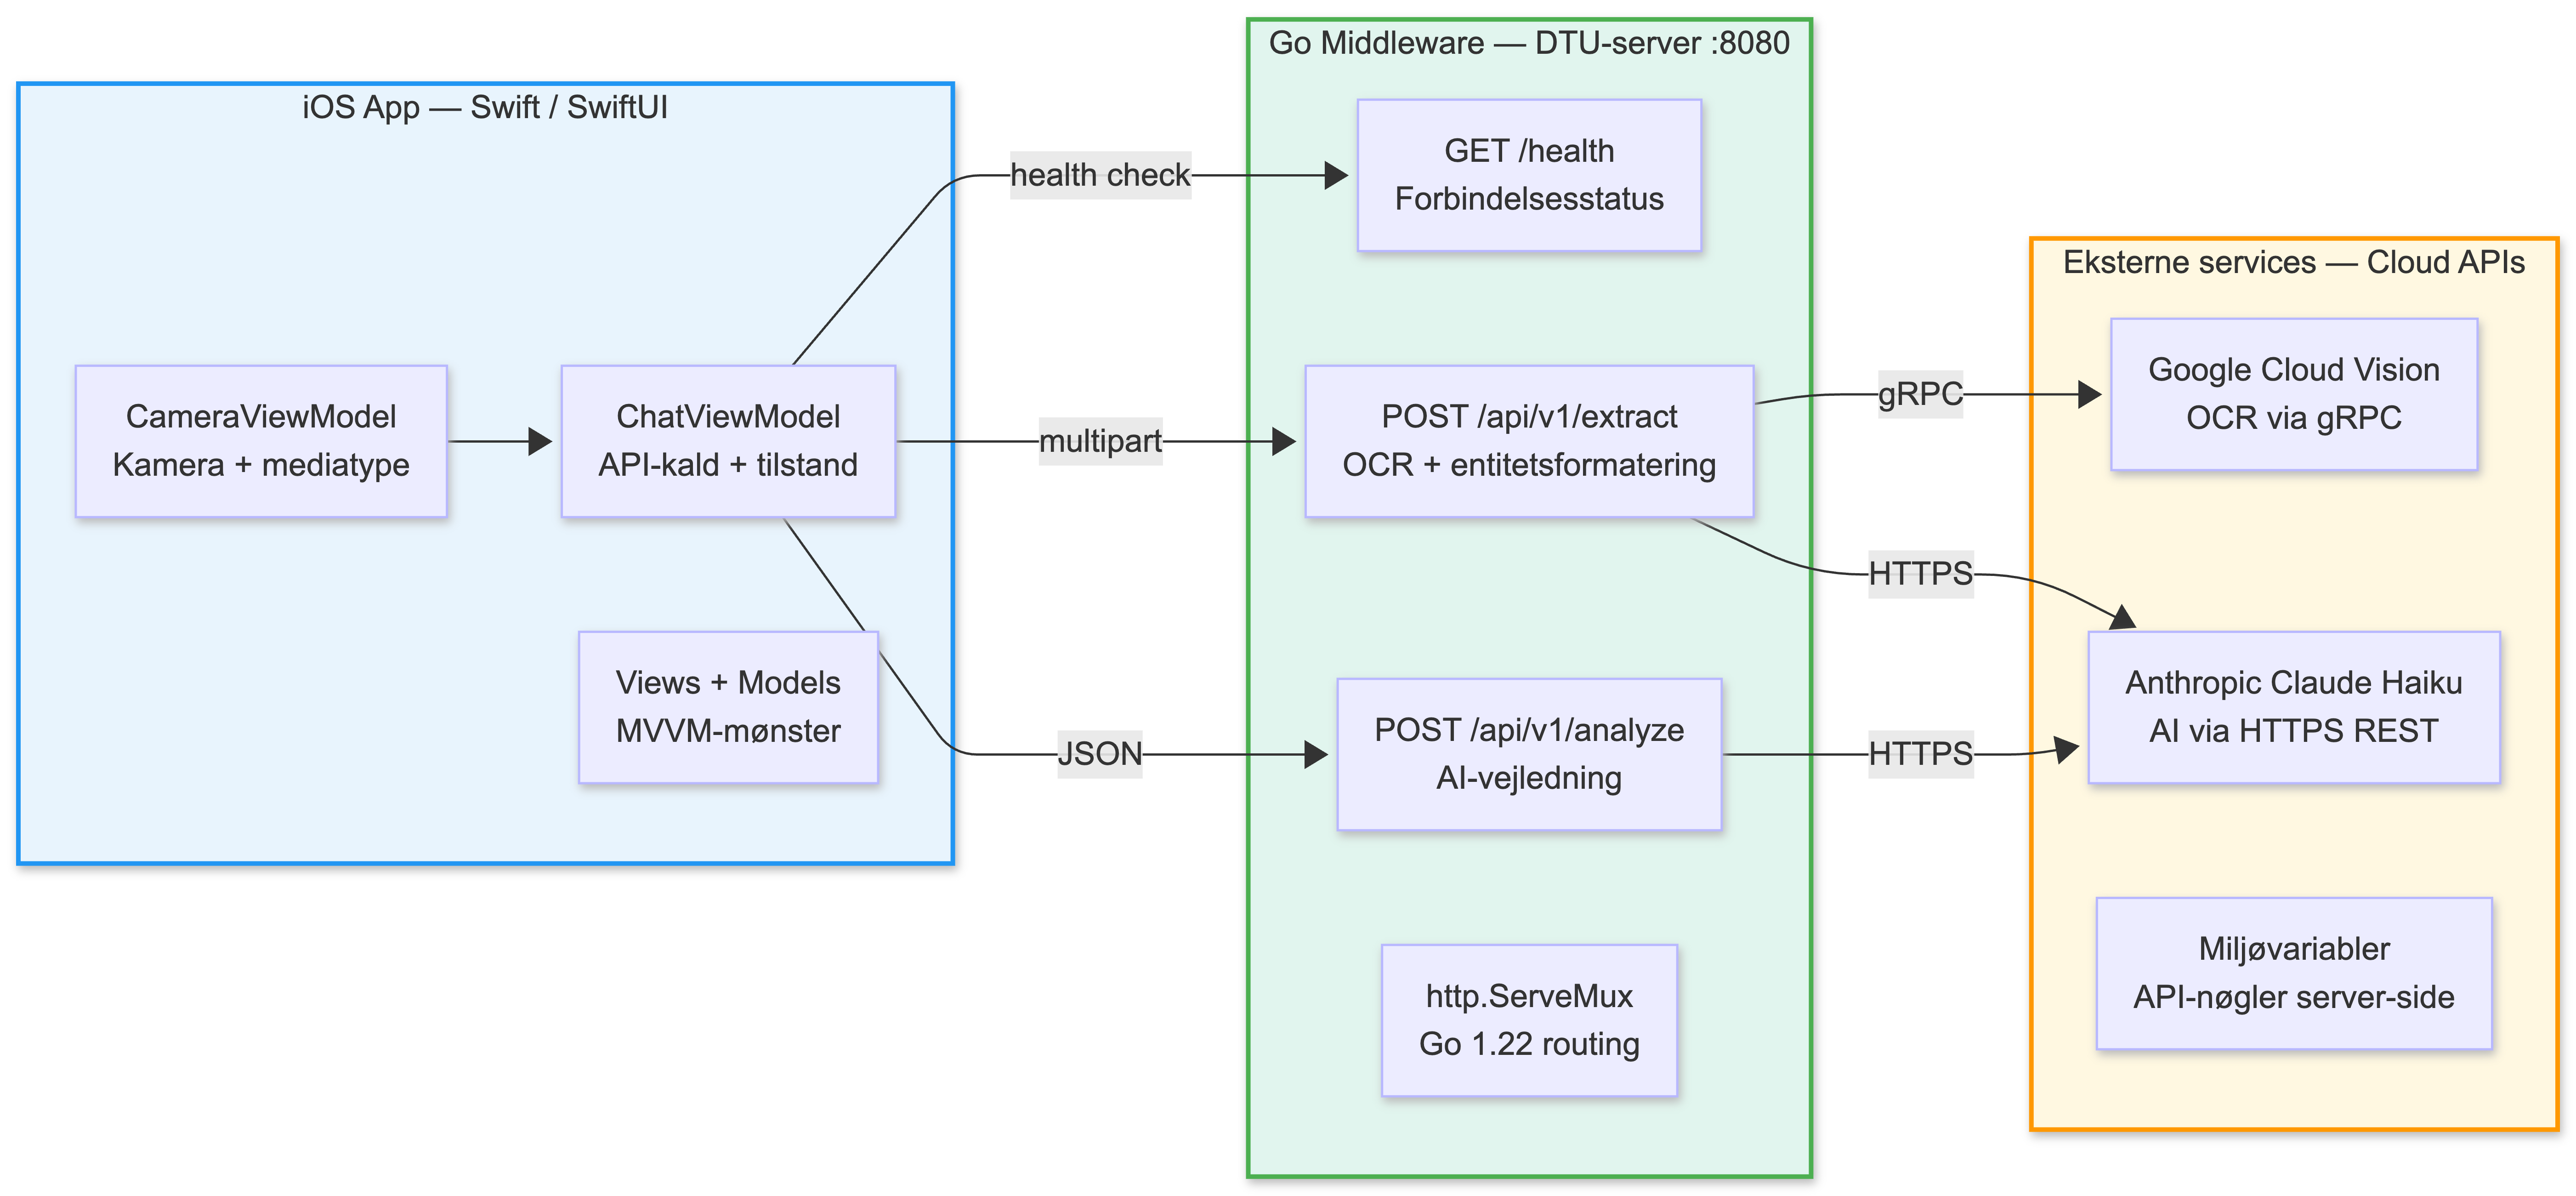
\includegraphics[width=\textwidth]{figures/Systemarkitektur.png}
  \caption{Overordnet systemarkitektur}
  \label{fig:system-overview}
\end{figure}


\textbf{iOS-applikationen} kører på teknikerens iPhone eller iPad og udgør brugergrænsefladen. Al logik i klientlaget er organiseret efter MVVM-mønstret (beskrevet i afsnit~\ref{sec:mvvm}). Kommunikation med serveren sker udelukkende via HTTP over det lokale netværk eller internet.

\textbf{Go middleware-serveren} er deployeret på en DTU-server (\texttt{130.225.170.229:8080}) og fungerer som det centrale orkestreringslag. Serveren modtager mediefiler fra klienten, koordinerer kald til eksterne AI-services og returnerer strukturerede svar til klienten. Ved at placere al AI-logik i middleware-laget undgås eksponering af API-nøgler i klientkoden, og det bliver muligt at udskifte individuelle services uden ændringer i iOS-applikationen.

\textbf{Google Cloud Vision} anvendes udelukkende til OCR-behandling af billeder og video-frames via gRPC-protokollen.

\textbf{Anthropic Claude Haiku} anvendes til to opgaver: strukturering af OCR-råtekst til typede entiteter og generering af vedligeholdelsesvejledning. Kommunikation sker via Anthropic's REST API over HTTPS.

\section{MVVM-arkitekturmønstret}
\label{sec:mvvm}

iOS-applikationen er struktureret efter MVVM-mønstret (Model-View-ViewModel), som adskiller brugergrænsefladen fra applikationens forretningslogik og datahåndtering~\cite{mvvm}. Figur~\ref{fig:mvvm} viser den konkrete mapping fra mønstret til applikationens komponenter.

\begin{figure}[H]
  \centering
  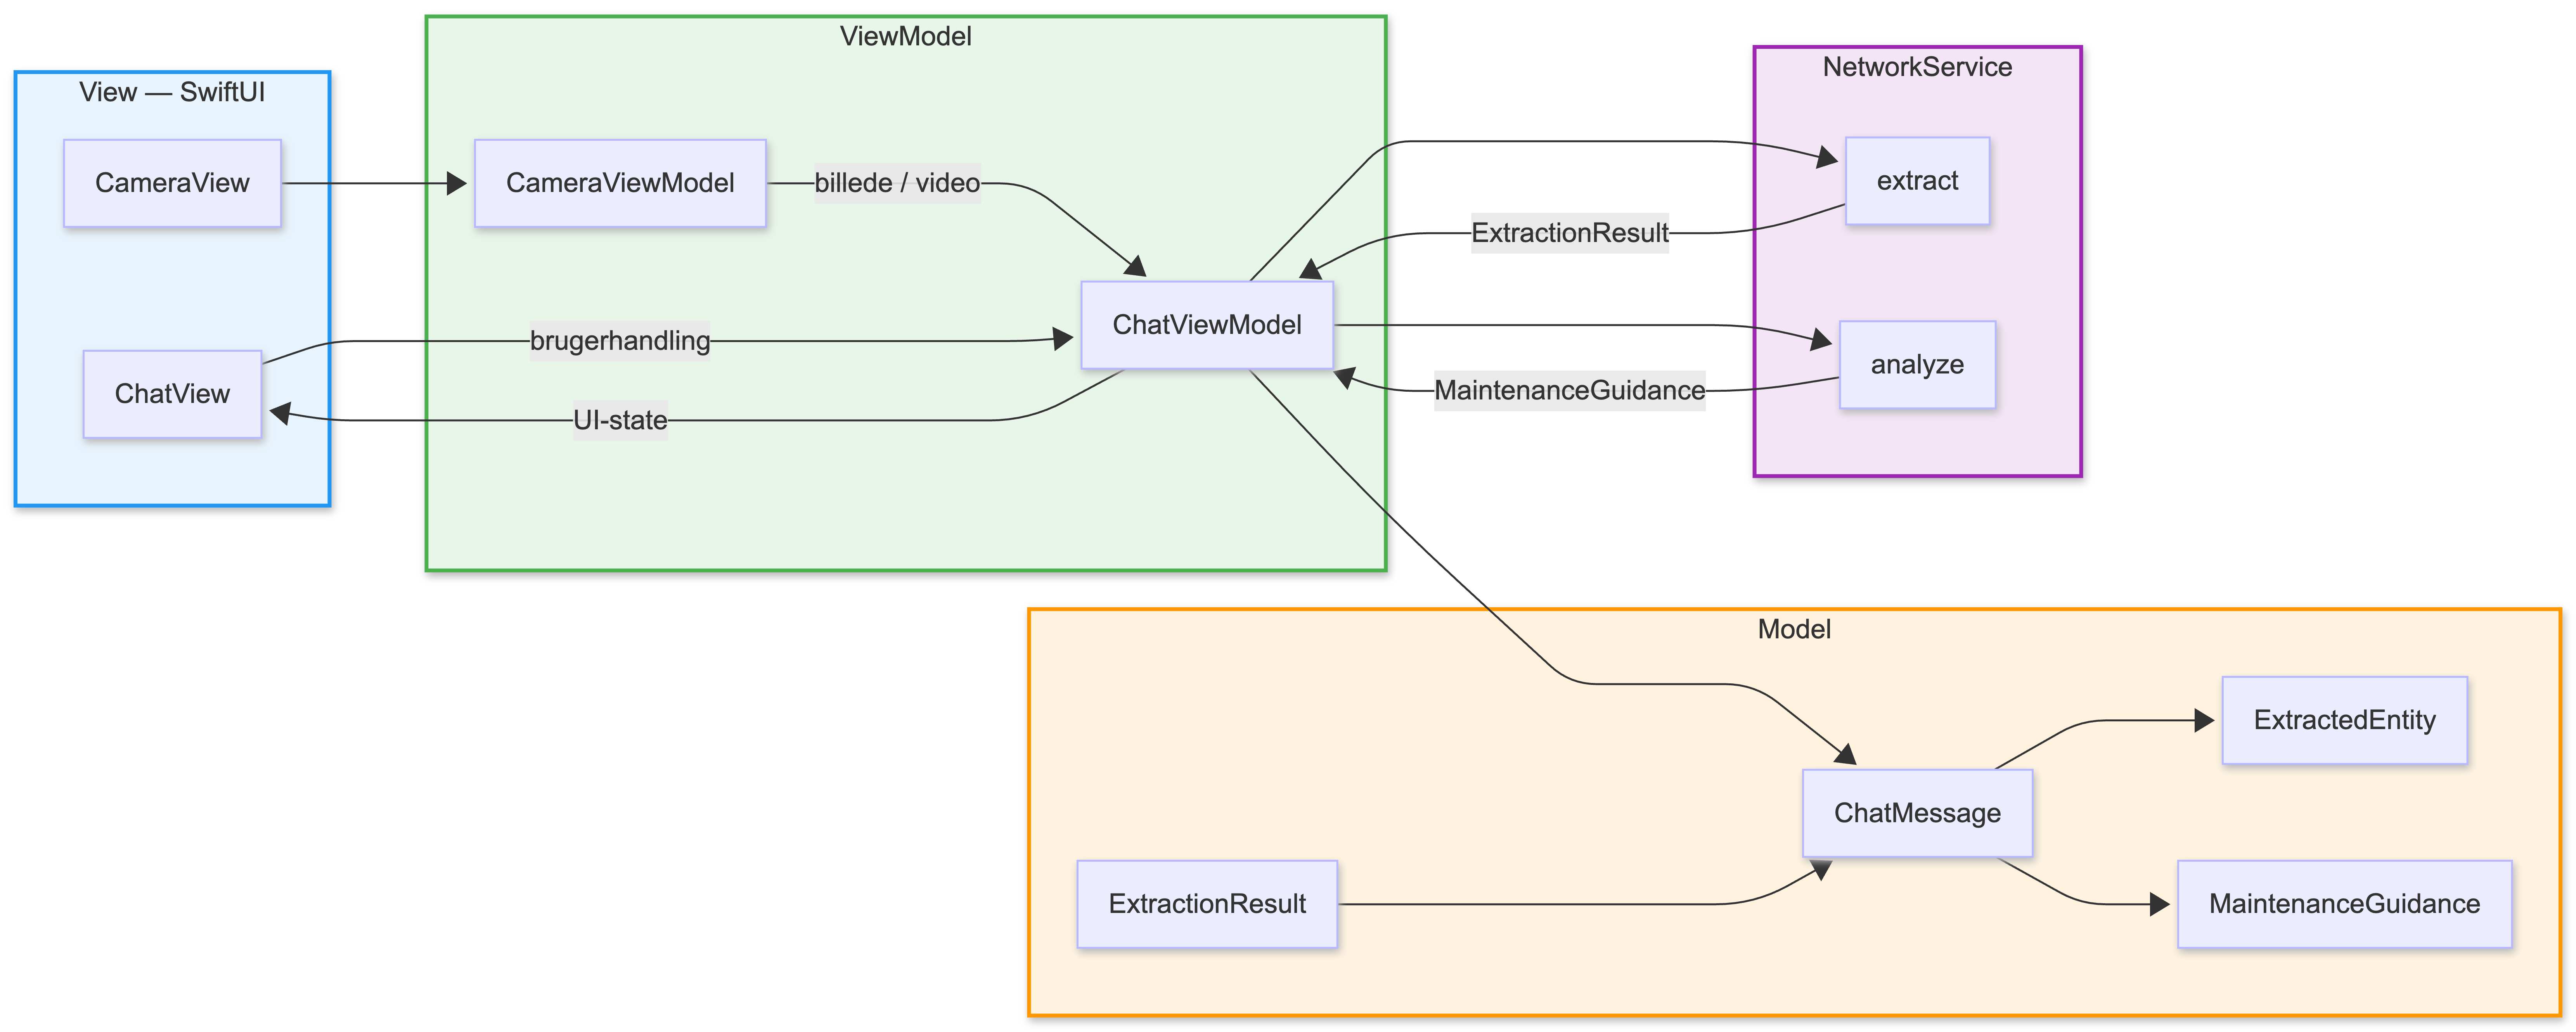
\includegraphics[width=0.85\textwidth]{figures/MVVM_final.png}
  \caption{MVVM-arkitektur i iOS-applikationen}
  \label{fig:mvvm}
\end{figure}

\textbf{Model-laget} repræsenterer applikationens datastrukturer. De centrale modeller er:

\begin{itemize}
  \item \texttt{ChatMessage} — en besked i chatten med en tilhørende \texttt{MessageKind}-enum der dækker seks tilstande: \texttt{text}, \texttt{extractedEntities}, \texttt{guidance}, \texttt{flagged}, \texttt{loading} og \texttt{error}
  \item \texttt{ExtractedEntity} — én identificeret entitet fra OCR-resultatet med label, værdi og tilladte handlinger
  \item \texttt{MaintenanceGuidance} — den strukturerede vedligeholdelsesvejledning returneret af Claude
  \item \texttt{ExtractionResult} — det samlede resultat af et extract-kald med entiteter, råtekst, confidence og review-flag
\end{itemize}

\textbf{ViewModel-laget} indeholder applikationens logik og fungerer som bindeled mellem View-laget og \texttt{NetworkService}:

\begin{itemize}
  \item \texttt{ChatViewModel} er annoteret med \texttt{@MainActor} og eksponerer \texttt{@Published}-properties til View-laget. ViewModellen implementerer et \textit{placeholder-replace-pattern}: når en netværksoperation startes, indsættes en loading-besked med et foruddefineret ID, som efterfølgende erstattes in-place af det endelige svar. Dette eliminerer flimmer i UI'et og bevarer beskedhistorikken intakt.
  \item \texttt{CameraViewModel} håndterer tilstanden for kamera-flowet, herunder valg af medie (billede eller video) og navigation til chat-visningen.
\end{itemize}

\textbf{NetworkService} fungerer som applikationens netværkslag og er det 
eneste sted der kommunikerer direkte med Go-middlewaren. \texttt{ChatViewModel} 
kalder \texttt{NetworkService.shared.extract()} og 
\texttt{NetworkService.shared.analyze()} via Swift's \texttt{async/await}, 
og \texttt{NetworkService} returnerer henholdsvis \texttt{ExtractionResult} 
og \texttt{MaintenanceGuidance} til \texttt{ChatViewModel}.


\textbf{View-laget} er implementeret i SwiftUI og består primært af \texttt{ChatView}, \texttt{CameraView} og et system af seks beskedbubble-typer, der renderer de forskellige \texttt{MessageKind}-tilstande.

\section{API-design}
\label{sec:api-design}

Middleware-serverens REST API eksponerer fire endpoints, som er opsummeret i tabel~\ref{tab:api-endpoints}.

\begin{table}[H]
  \centering
  \caption{API-endpoints på Go middleware-serveren}
  \label{tab:api-endpoints}
  \begin{tabularx}{\textwidth}{@{}llX@{}}
    \toprule
    \textbf{Metode} & \textbf{Endpoint} & \textbf{Beskrivelse} \\
    \midrule
    \texttt{GET}  & \texttt{/health}          & Returnerer serverens status og tidsstempel. Anvendes af iOS-klienten til at vise forbindelsesstatus i realtid \\
    \addlinespace
    \texttt{GET}  & \texttt{/version}         & Returnerer API-versionsnummer \\
    \addlinespace
    \texttt{POST} & \texttt{/api/v1/extract}  & Modtager et billede eller en video som \texttt{multipart/form-data}, kører OCR og returnerer strukturerede entiteter som JSON \\
    \addlinespace
    \texttt{POST} & \texttt{/api/v1/analyze}  & Modtager en valgt entitet med kontekst som JSON og returnerer struktureret vedligeholdelsesvejledning \\
    \bottomrule
  \end{tabularx}
\end{table}

Routingen implementeres via Go 1.22's indbyggede \texttt{http.ServeMux} med method-prefixed patterns, eksempelvis \texttt{"POST /api/v1/extract"}, hvilket eliminerer behovet for tredjeparts routing-biblioteker og giver klar adskillelse af HTTP-metoder på compilerniveau.

\section{Dataflow: Billedbaseret udtræk}
\label{sec:dataflow-billede}

Figur~\ref{fig:flow-image} viser det komplette dataflow for det primære use case: upload af et billede og udtræk af maskinentiteter.

\begin{figure}[H]
  \centering
  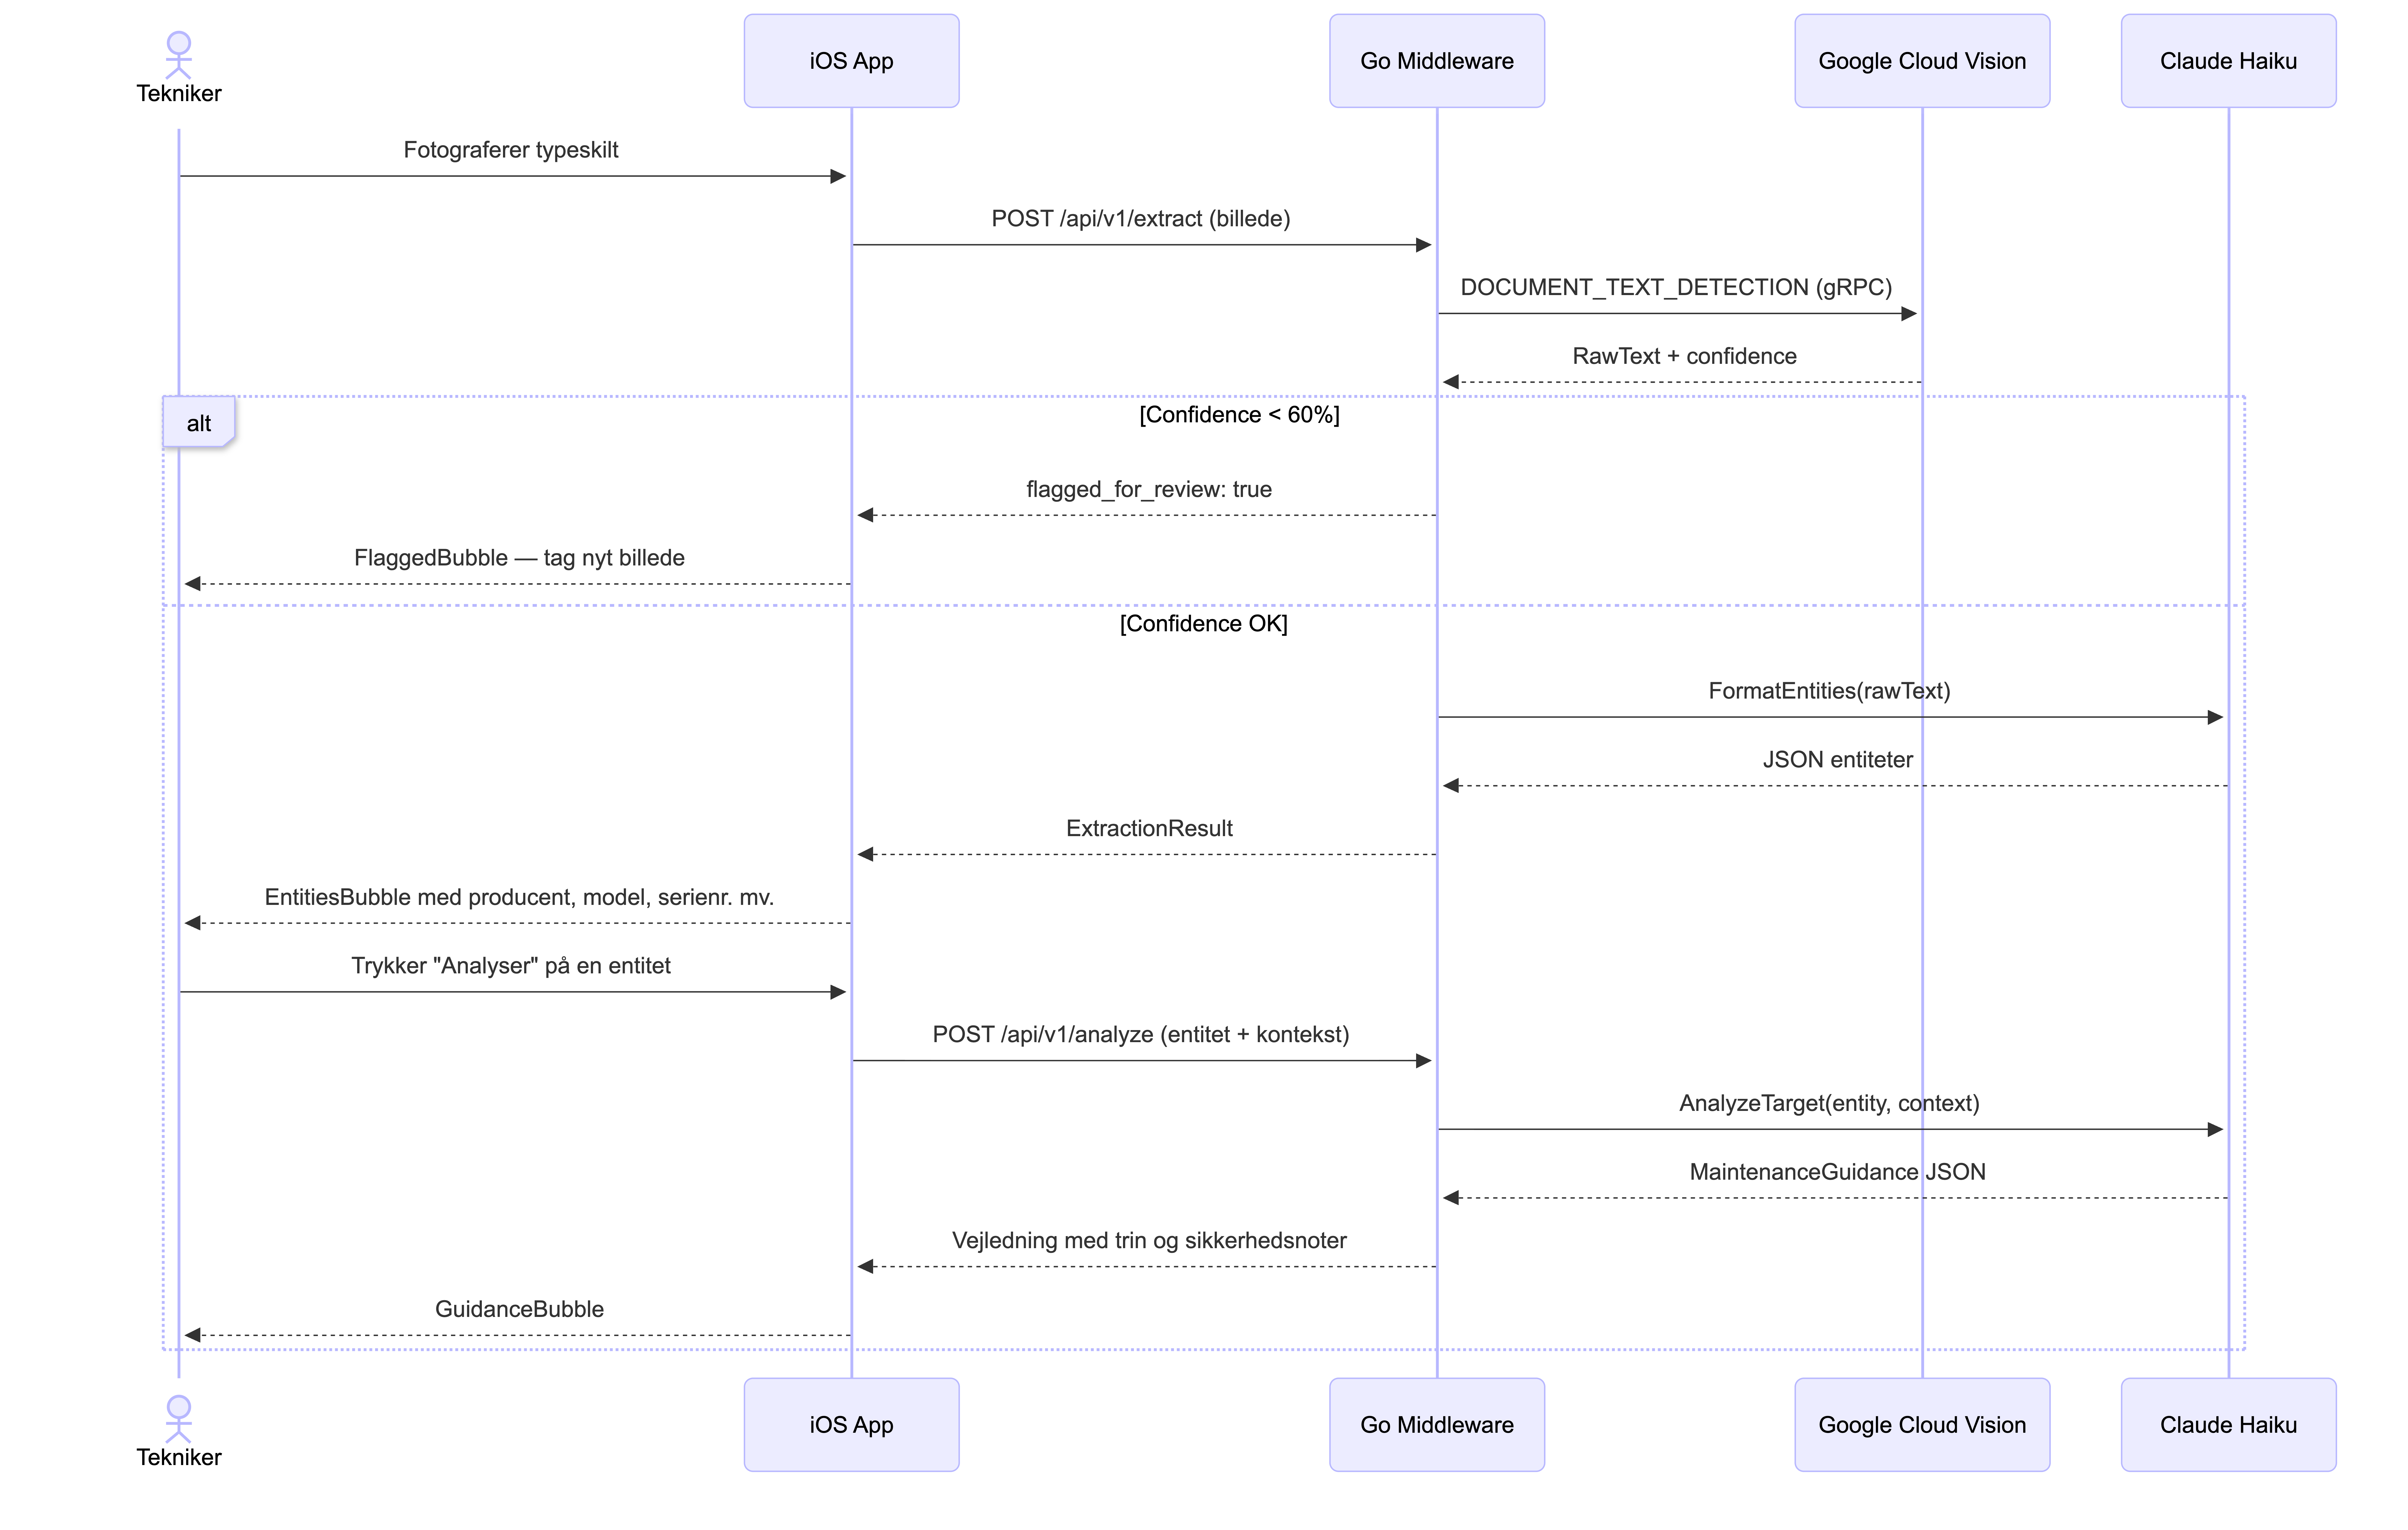
\includegraphics[width=\textwidth]{figures/AppFlowDiagram.png}
  \caption{Sekvensdiagram for billedbaseret udtræk}
  \label{fig:flow-image}
\end{figure}

Forløbet er som følger:

\begin{enumerate}
  \item Teknikeren optager et billede via \texttt{ImagePicker}, som returnerer et \texttt{UIImage}-objekt til \texttt{CameraViewModel}
  \item \texttt{ChatViewModel.extractImage()} konverterer billedet til JPEG-data (80\% komprimering) og sender det som \texttt{multipart/form-data} til \texttt{POST /api/v1/extract} med en timeout på 60 sekunder
  \item \texttt{NewExtractHandler} i Go parser form-data og sender billedets rå bytes til Google Cloud Vision via \texttt{BatchAnnotateImages}-kaldet med \texttt{DOCUMENT\_TEXT\_DETECTION}-feature
  \item Vision returnerer en \texttt{FullTextAnnotation} med tekst og symbol-confidence scores. Funktionen \texttt{averageSymbolConfidence()} traverserer annotationshierarkiet (side → blok → paragraf → ord → symbol) og beregner en gennemsnitlig confidence-score
  \item Hvis confidence er under tærsklen på 60\% (\texttt{confidenceThreshold = 0.60}), returneres resultatet øjeblikkeligt med \texttt{FlaggedForReview: true} uden at kalde Claude
  \item Ved tilstrækkelig confidence sendes råteksten til \texttt{ClaudeClient.FormatEntities()}, som via \texttt{extractSystemPrompt} instruerer modellen til at returnere strukturerede entiteter som JSON
  \item \texttt{cleanJSONResponse()} udtrækker JSON-objektet fra svaret og trimmer eventuelle markdown-wrappers
  \item Det dekodede \texttt{ExtractionResult} returneres til iOS-klienten, som renderer resultatet som en \texttt{EntitiesBubble} eller — ved lav confidence — en \texttt{FlaggedBubble}
\end{enumerate}

\section{Dataflow: Videobaseret udtræk}
\label{sec:dataflow-video}

Videobehandlingen følger et udvidet pipeline der inkluderer frame-udtræk via ffmpeg:

\begin{enumerate}
  \item Teknikeren optager en video og panorerer kameraet henover maskinlabelen. Videofilen (mp4-format) sendes som \texttt{multipart/form-data} til \texttt{POST /api/v1/extract} med en timeout på 120 sekunder
  \item \texttt{processVideo()} i \texttt{video.go} gemmer videodata i en midlertidig mappe og kalder ffmpeg via \texttt{exec.CommandContext}: \texttt{ffmpeg -i video.mp4 -vf fps=1 frame\_\%03d.jpg}
  \item Hvert ekstraheret frame sendes individuelt til Google Cloud Vision OCR
  \item Tekstresultaterne fra alle frames aggregeres med frame-headers (\texttt{"--- Frame N ---"}) og en gennemsnitlig confidence beregnes på tværs af alle gyldige frames
  \item Det aggregerede tekstindhold behandles af Claude som én samlet streng, identisk med billedflowet
\end{enumerate}

Den midlertidige mappe slettes automatisk via \texttt{defer os.RemoveAll(tempDir)} uanset udfaldet af behandlingen.

\section{Dataflow: AI-vejledning}
\label{sec:dataflow-analyze}

Når teknikeren trykker \textit{Analyser} på en entitet i \texttt{EntitiesBubble}, trigges følgende flow:

\begin{enumerate}
  \item \texttt{ChatViewModel.analyzeEntity()} sender en \texttt{AnalyzeRequest} som JSON til \texttt{POST /api/v1/analyze} med \texttt{target\_label}, \texttt{target\_value}, \texttt{machine\_model} (udledt fra kontekst-entiteterne) og alle øvrige entiteter som baggrundskontekst
  \item \texttt{NewAnalyzeHandler} validerer input og videresender til \texttt{ClaudeClient.AnalyzeTarget()}
  \item Claude instrueres via \texttt{analyzeSystemPrompt} til at generere struktureret vejledning med minimum tre vejledningsskridt, to sikkerhedsnoter og et \texttt{uncertainty\_level} (\texttt{"low"}, \texttt{"medium"} eller \texttt{"high"})
  \item Sproget for vejledningen styres af \texttt{language}-feltet i requesten (\texttt{"da"} eller \texttt{"en"}), som bestemmer hvilken sproglig instruktion der tilføjes prompten
  \item Den dekodede \texttt{MaintenanceGuidance} returneres og renderes som en \texttt{GuidanceBubble} i iOS-klienten
\end{enumerate}

\section{Fejlhåndtering}
\label{sec:fejlhaandtering}

Systemet implementerer en gennemgående fejlhåndteringsstrategi på tværs af klient og server.

På \textbf{serversiden} returnerer alle handlers strukturerede JSON-fejlsvar med HTTP-statuskoder. Input valideres eksplicit inden AI-kald, så ugyldige requests afvises med \texttt{400 Bad Request} før eksterne services kontaktes.

På \textbf{klientsiden} implementerer \texttt{ChatViewModel} et \texttt{RetryContext}-mønster: enhver fejlbesked gemmer den originale kontekst (billeddata, video-URL eller entitet), så brugeren kan prøve igen med ét tryk uden at gentage hele flowet fra start. Dette håndteres via \texttt{ErrorBubble}-komponenten, der viser en meningsfuld fejlbesked og en \textit{Prøv igen}-knap.

\section{Deployment}
\label{sec:deployment}

Go-serveren deployes til DTU-serveren via et automatiseret shell-script (\texttt{deploy.sh}), der udfører følgende trin i rækkefølge:

\begin{enumerate}
  \item Køring af samtlige Go-unit tests (\texttt{go test ./...}) — scriptet afbrydes ved testfejl
  \item Cross-kompilering til Linux/amd64: \texttt{GOOS=linux GOARCH=amd64 go build -o arkyn-server}
  \item Stop af den kørende systemd-service via SSH
  \item Kopiering af den nye binær til serveren via \texttt{scp}
  \item Genstart af service og verifikation af servicestatus
\end{enumerate}

Serverens konfiguration — herunder API-nøgler til Anthropic og Google Cloud — læses udelukkende fra miljøvariabler (\texttt{ANTHROPIC\_API\_KEY}, \texttt{GOOGLE\_APPLICATION\_CREDENTIALS}), der aldrig indgår i versionsstyringen.

\chapter{UI/UX Design}
\label{chap:ux}

\section{Målgruppe og designrationale}
\label{sec:målgruppe}

Applikationens primære brugere er vedligeholdelsesteknikere, der arbejder i industrielle produktionsmiljøer. En central observation fra behovskortlægningen i samarbejde med Arkyn Studios er, at en væsentlig del af denne brugergruppe udgøres af ældre herrer og kvinder, der ikke nødvendigvis har daglig erfaring med at betjene en iPad eller andre touchbaserede enheder. Mange er erfarne fagfolk med betydelig teknisk viden om maskiner og udstyr, men deres digitale fortrolighed varierer markant.

Dette stiller særlige krav til designet. Det er ikke tilstrækkeligt at designe en applikation, der blot er funktionel — den skal være så intuitiv, at en bruger uden erfaring med mobile applikationer kan gennemføre kerneflowet fra kameraåbning til AI-genereret vejledning uden forudgående oplæring. Designfilosofien har derfor fra starten været at holde brugergrænsefladen så simpel og direkte som mulig: færre valg ad gangen, tydelige handlinger og ingen unødvendig kompleksitet.

Denne tilgang er i overensstemmelse med krav NF4 fra kravspecifikationen, som eksplicit fastslår, at kerneflowet skal kunne gennemføres uden forudgående instruktion.

\section{Designprincipper}
\label{sec:designprincipper}

Designet er bygget op om tre overordnede principper, der alle understøtter den brede og varierede brugergruppe.

\textbf{Simpelt og lineært brugerflow.} Applikationen er organiseret omkring ét enkelt, lineært kerneflow: tag et billede $\rightarrow$ gennemgå de udtrukne data $\rightarrow$ modtag vedligeholdelsesvejledning. Brugeren præsenteres aldrig for mere end ét primært handlingsvalg ad gangen. Dette reducerer kognitiv belastning og minimerer risikoen for at navigere forkert — et hensyn der er særligt vigtigt for brugere med begrænset erfaring med touchskærme.

\textbf{Store, tydelige interaktionselementer.} Knapper og trykflader er dimensioneret med generøs tapstørrelse for at imødekomme brugere, der måske er uvante med berøringsskærme eller arbejder med handsker på. Tekst er valgt i en let læselig skriftstørrelse, og farvekontrasten er høj nok til at sikre god læsbarhed selv i industrielle lysforhold med direkte sollys eller kunstig belysning.

\textbf{Meningsfuld og umiddelbar feedback.} Brugeren holdes løbende orienteret om systemets tilstand via synlige loading-indikatorer og kortfattede statusbeskeder. Fejlsituationer — eksempelvis lav OCR-kvalitet eller netværksproblemer — kommunikeres i klart og handlingsorienteret sprog frem for tekniske fejlkoder, så brugeren altid ved, hvad det næste skridt er.

Disse principper afspejler Nielsens klassiske usability-heuristikker~\cite{nielsen_heuristics}, særligt \textit{Visibility of system status}, \textit{Error prevention} og \textit{Recognition rather than recall}, der alle sigter mod at reducere brugerens mentale arbejdsbyrde.

\section{Navigation og informationsarkitektur}
\label{sec:navigation}

Applikationen er struktureret som en \texttt{TabView} med to primære faner: \textbf{Kamera} og \textbf{Chat}. Denne fladstruktur er et bevidst designvalg. En dybere navigationshierarki med undermapper og indstillingssider ville øge kompleksiteten unødvendigt for en brugergruppe, der primært har ét formål med applikationen: at identificere en maskine og modtage vejledning hurtigt.

Fanestrukturen giver brugeren et øjeblikkeligt overblik over de tilgængelige funktioner og eliminerer behovet for at huske, hvor en specifik funktion befinder sig. Dette er et vigtigt hensyn for brugere, der kun åbner applikationen sporadisk i forbindelse med vedligeholdelsesopgaver.

\section{Chat-interface og bobledesign}
\label{sec:chatdesign}

Interaktionen med systemet er modelleret som en chat-samtale, hvilket er en velkendt paradigme for en bred brugergruppe. Resultater præsenteres som meddelelsesbob\-ler (\textit{bubbles}), der er differentieret visuelt efter indholdstype:

\begin{itemize}
  \item \textbf{EntitiesBubble} viser de strukturerede data, der er udtrukket fra maskinlabelen via OCR. Hvert felt præsenteres med tilhørende handlingsknapper (kopiér, søg, analyser), der giver brugeren kontrol over næste skridt.
  \item \textbf{GuidanceBubble} præsenterer den AI-genererede vedligeholdelsesvejledning med tydelig opdeling i handlingstrin, sikkerhedsadvarsler og kildehenvisninger.
  \item \textbf{FlaggedBubble} anvendes når OCR-confidence er under tærsklen på 60~\%. Boblen informerer brugeren klart om årsagen og opfordrer til at tage et nyt billede.
  \item \textbf{ErrorBubble} håndterer netværksfejl og API-timeouts med en synlig rød farvemarkering og en \textit{Prøv igen}-knap, der lader brugeren gentage handlingen med ét tryk.
  \item \textbf{LoadingHintBubble} vises under API-kald og kommunikerer systemets tilstand med en kort beskrivelse og en animeret tre-prikkers indikator.
\end{itemize}

Denne differentiering sikrer, at brugeren altid kan skelne mellem systemets tilstande uden at skulle læse teknisk information.

\section{Kameraoverlay og videooptagelse}
\label{sec:kameraoverlay}

For at guide brugeren under optagelsen er der implementeret et kameraoverlay, der vises i de første seks sekunder. Overlayet indeholder en kort instruktion om at panorere kameraet fra venstre mod højre for store labels, og forsvinder automatisk, inden brugeren begynder optagelsen. Dette er et eksempel på, at systemet proaktivt reducerer brugerens behov for at huske instruktioner.

Overlayet er implementeret via \texttt{UIHostingController} med \texttt{isUserInteractionEnabled = false}, hvilket sikrer, at berøringsinput passerer igennem til kameraets egne kontrolflader uden forstyrrelser.

\section{Sprogunderstøttelse}
\label{sec:sprog}

Applikationen understøtter skift mellem dansk og engelsk vejledning via en globusknap i navigationslinjen i chat-visningen. Valget persisteres via \texttt{@AppStorage}, og sendes med i hvert API-kald til backenden, der derefter instruerer Claude-modellen til at generere vejledning på det ønskede sprog. Dette imødekommer kravet F7 og giver virksomheder med internationale teknikere mulighed for at anvende applikationen på begge sprog.

\chapter{Implementering}
\label{chap:implementation}

Dette kapitel beskriver den tekniske implementering af systemets to hoveddele: iOS-frontenden udviklet i Swift og SwiftUI, samt Go-middlewaren der orkestrerer kommunikationen mellem klienten og de eksterne AI-services.

\section{Frontend — Swift og SwiftUI}
\label{sec:frontend}

Frontenden er implementeret i Swift med SwiftUI som UI-framework. SwiftUI's deklarative tilgang passer naturligt til den komponentbaserede struktur, som designprincipperne foreskriver. Tilstandsstyringen følger MVVM-arkitekturmønstret~\cite{mvvm}, hvor \texttt{ViewModel}-laget håndterer al logik og kommunikation med backenden, mens \texttt{View}-laget udelukkende er ansvarligt for præsentationen.

\subsection{Arkitektur og MVVM}
\label{subsec:mvvm}

Applikationens centrale \texttt{ViewModel} er \texttt{ChatViewModel}, der er markeret med \texttt{@MainActor} for at sikre, at alle UI-opdateringer sker på main-tråden. Klassen eksponerer en \texttt{@Published}-liste af \texttt{ChatMessage}-objekter, som SwiftUI automatisk reagerer på og gengiver. \texttt{ChatMessage} er en value type med et \texttt{MessageKind}-enum, der dækker alle mulige tilstande: \texttt{text}, \texttt{extractedEntities}, \texttt{guidance}, \texttt{flagged}, \texttt{loading} og \texttt{error}.

Denne tilstandsmodel gør det muligt at erstatte en loading-boble in-place med det endelige svar, uden at indsætte et nyt element i listen. Det eliminerer flimmer i brugergrænsefladen og giver en naturlig chat-oplevelse:

\begin{lstlisting}[language=Swift, caption={In-place erstatning af loading-besked i ChatViewModel}]
if let idx = messages.firstIndex(where: { $0.id == placeholderId }) {
    messages[idx] = result
    scrollTrigger += 1
}
\end{lstlisting}

\subsection{Kameraintegration og mediatyper}
\label{subsec:kamera}

Kameraintegration er implementeret via \texttt{UIImagePickerController} i en \texttt{UIViewControllerRepresentable}-wrapper ved navn \texttt{ImagePicker}. Komponenten understøtter både stillbilleder og videooptagelse ved at sætte \texttt{mediaTypes} til at inkludere både \texttt{UTType.image} og \texttt{UTType.movie}.

Mediatypen afspejles i en \texttt{MediaType}-enum i \texttt{CameraViewModel}, der skelner mellem \texttt{image(UIImage)} og \texttt{video(URL)}. Denne skelnen er central for, hvilket API-endpoint der efterfølgende kaldes: billeder sendes til \texttt{/api/v1/extract} som JPEG-data, mens videoer uploades som rå \texttt{.mp4}-filer og behandles af serverens video-pipeline.

\subsection{Fejlhåndtering og retry-mekanisme}
\label{subsec:retry}

Fejlhåndteringen er bygget op om en \texttt{RetryContext}-enum, der indeholder al nødvendig information til at gentage en fejlet handling. Når brugeren trykker \textit{Prøv igen} på en \texttt{ErrorBubble}, kaldes \texttt{ChatViewModel.retry(messageId:context:)}, der genkender konteksten og kalder det korrekte endpoint igen — med den originale loading-boble erstattet frem for en ny tilføjet:

\begin{lstlisting}[language=Swift, caption={Retry-mekanisme baseret på RetryContext}]
func retry(messageId: UUID, context: RetryContext) async {
    switch context {
    case .extractImage(let imageData):
        await extractImage(imageData, replaceMessageId: messageId)
    case .extractVideo(let videoURL):
        await extractVideo(videoURL, replaceMessageId: messageId)
    case .analyzeEntity(let entity, let context):
        await analyzeEntity(entity, context: context,
                            replaceMessageId: messageId)
    case .sendChatMessage(let text, let imageData):
        currentMessage = text
        await sendMessage(withImage: imageData,
                         replaceMessageId: messageId)
    }
}
\end{lstlisting}

\section{Backend — Go og middleware-pipeline}
\label{sec:backend}

Backenden er implementeret som en Go-baseret middleware-service, der fungerer som orkestrerende lag mellem iOS-klienten og de eksterne AI-services. Valget af Go er begrundet i sprogets lave latens, enkle concurrency-model via goroutines og den kompakte deploymentflade, der er velegnet til en prototype~\cite{go_docs}.

Serveren eksponerer fire HTTP-endpoints via \texttt{net/http}'s standard multiplexer:

\begin{table}[H]
  \centering
  \caption{API-endpoints}
  \label{tab:endpoints}
  \begin{tabularx}{\textwidth}{@{}llX@{}}
    \toprule
    \textbf{Metode} & \textbf{Sti} & \textbf{Beskrivelse} \\
    \midrule
    GET  & \texttt{/health}          & Returnerer serverens tilstand og tidsstempel \\
    \addlinespace
    GET  & \texttt{/version}         & Returnerer den aktuelle API-version \\
    \addlinespace
    POST & \texttt{/api/v1/extract}  & Modtager billede eller video, kører OCR og returnerer strukturerede entiteter \\
    \addlinespace
    POST & \texttt{/api/v1/analyze}  & Modtager en entitet og returnerer AI-genereret vedligeholdelsesvejledning \\
    \bottomrule
  \end{tabularx}
\end{table}

\subsection{Extract-pipeline}
\label{subsec:extract}

\texttt{/api/v1/extract} er systemets primære indgangspunkt og håndterer begge mediatyper. Handleren følger dette forløb:

\begin{enumerate}
  \item Multipart-formen parses med en øvre grænse på 50~MB for at understøtte videoer.
  \item Afhængigt af om feltet \texttt{image} eller \texttt{video} er til stede, vælges den tilsvarende OCR-sti.
  \item For billeder sendes bytes direkte til Google Cloud Vision via \texttt{DOCUMENT\_TEXT\_DETECTION}.
  \item For videoer ekstraheres frames med \texttt{ffmpeg} ved 1 FPS, hvorefter OCR køres på hvert enkelt frame, og resultatteksten aggregeres.
  \item Hvis den gennemsnitlige confidence er under 60~\%, returneres svaret med \texttt{flagged\_for\_review: true} uden at kalde Claude.
  \item Ellers sendes den rå OCR-tekst til Claude Haiku, der formaterer den til strukturerede JSON-entiteter med tilhørende handlingstyper.
\end{enumerate}

\subsection{Analyze-pipeline}
\label{subsec:analyze}

\texttt{/api/v1/analyze} modtager den entitet, brugeren har valgt at analysere, samt kontekstentiteterne fra extract-steget. Claude Haiku instrueres via en fastlåst system-prompt til at returnere et JSON-objekt med felterne \texttt{general\_guidance}, \texttt{safety\_notes}, \texttt{source\_references} og \texttt{uncertainty\_level}. Sprogvalget — dansk eller engelsk — videregives fra iOS-klienten og oversættes til en eksplicit sprogbetingelse i prompten.

\subsection{Valg af Claude Haiku frem for alternativer}
\label{subsec:claude-valg}

I forbindelse med valget af AI-model blev Anthropic Claude Haiku~\cite{anthropic_claude} valgt frem for sammenlignelige alternativer som OpenAI GPT-4o Mini. Valget er baseret på tre faktorer:

\textbf{Lavere hallucinationsrate.} Anthropics Constitutional AI-metode~\cite{anthropic_claude} er designet til at minimere situationer, hvor modellen opfinder information, der ikke er til stede i inputtet — et kritisk krav i en vedligeholdelseskontekst, hvor forkerte instruktioner kan medføre sikkerhedsrisici.

\textbf{Struktureret JSON-output.} Claude Haiku følger stringent strukturerede promptinstruktioner og returnerer konsekvent validt JSON, hvilket forenkler parsing-laget i Go-middlewaren og reducerer behovet for defensiv fejlhåndtering.

\textbf{Naturlig synergi med OCR-workflow.} Kombinationen af Google Cloud Vision og Claude Haiku giver en veldefineret to-trins pipeline: Vision udtrækker teksten, Claude strukturerer og fortolker den. Da begge services leverer veldokumenterede REST-API'er, holdes integrationskompleksiteten lav.

\subsection{Sikring af API-nøgler}
\label{subsec:sikkerhed}

I overensstemmelse med krav NF6 indgår ingen API-nøgler i klientkoden eller versionsstyringen. Nøglerne til Anthropic og Google Cloud Vision indlæses udelukkende fra miljøvariabler på serveren via en \texttt{config}-pakke, der terminerer programmet ved opstart, hvis nøglerne ikke er sat. På serveren gemmes nøglerne i en \texttt{.env}-fil, der er eksplicit ekskluderet fra Git-historikken.

\section{Deployment}
\label{sec:deployment}

Backenden er deployet på en DTU-server (\texttt{130.225.170.229:8080}) som en Linux-systemtjeneste administreret via \texttt{systemd}. Et dedikeret deploy-script (\texttt{deploy.sh}) automatiserer hele processen: det kører de lokale Go-tests, cross-kompilerer til Linux/amd64, kopierer binæren via SSH og genstarter tjenesten. Dette sikrer, at deploys kun sker, når alle tests er grønne, og at serveren altid kører en verificeret build.

\begin{lstlisting}[language=bash, caption={Uddrag af deploy-scriptets kernetrin}]
# Kør lokale tests – stopper scriptet ved fejl
go test ./...

# Cross-kompilér til Linux
GOOS=linux GOARCH=amd64 go build -o arkyn-server ./cmd/server/

# Stop service, kopiér binær, genstart
ssh "$SERVER" "sudo systemctl stop arkyn"
scp "$LOCAL_MIDDLEWARE/arkyn-server" "$SERVER:~/arkyn-middleware/.../arkyn-server"
ssh "$SERVER" "sudo systemctl restart arkyn"
\end{lstlisting}

\chapter{Test og evaluering}
\label{chap:testing}

Dette kapitel beskriver den testindsats der er gennemført for at verificere systemets funktionalitet og brugbarhed. Testningen kombinerer automatiserede enhedstests af backend-endpoints med manuel funktionstest og en bredere empirisk evaluering med fysiske maskinlabels og billeder fra varierende kilder.

\section{Testmiljø og teststrategi}
\label{sec:testmiljø}

For at sikre, at ny kode er funktionel inden den pushes til produktionsserveren på DTU, er der etableret et lokalt testmiljø, der spejler serveropsætningen. Testmiljøet kører Go-backenden lokalt på port 8080 og er konfigureret med de samme miljøvariabler som produktionsmiljøet. Dette giver mulighed for at validere ændringer isoleret, inden de deployes via det automatiserede deploy-script.

Teststrategien kombinerer tre niveauer:

\begin{enumerate}
  \item \textbf{Enhedstest} af backend-handlers via Go's standardtestframework
  \item \textbf{Manuel funktionstest} af den samlede pipeline med reelle billeder og videoer
  \item \textbf{Empirisk evaluering} af OCR-nøjagtighed og AI-vejledningskvalitet på tværs af forskelligartede testmaterialer
\end{enumerate}

\section{Enhedstest}
\label{sec:enhedstest}

Backend-endpoints er dækket af enhedstests implementeret i Go's \texttt{testing}-pakke. Tests køres lokalt som en del af deploy-flowet og vil stoppe en deployment, hvis de fejler.

\subsection{Health- og version-endpoints}
\label{subsec:health-test}

\texttt{TestHealthHandler} verificerer, at \texttt{GET /health} returnerer HTTP 200 og en ikke-tom JSON-body. \texttt{TestVersionHandler} verificerer tilsvarende, at \texttt{GET /version} returnerer HTTP 200 og et ikke-tomt \texttt{version}-felt i JSON-svaret. Begge tests anvender \texttt{httptest.NewRecorder} til at kalde handleren direkte uden en reel HTTP-server.

\subsection{Validering af extract-handler}
\label{subsec:extract-test}

\texttt{TestExtractHandler\_Validation} dækker to negative testcases:

\begin{itemize}
  \item \textbf{Missing Multipart Form:} En request med \texttt{Content-Type: text/plain} sendes til \texttt{/api/v1/extract}. Handleren forventes at returnere HTTP 400, inden den forsøger at kontakte OCR- eller AI-servicen.
  \item \textbf{Missing Image Field:} En korrekt multipart-form sendes, men uden et \texttt{image}-felt. Handleren forventes at returnere HTTP 400.
\end{itemize}

I begge cases sendes \texttt{nil} ind som Vision- og Claude-klient. Hvis valideringen fejler og koden forsøger at kontakte servicene, vil testen crashe med en panic, der beviser at valideringen er utilstrækkelig.

\subsection{Validering af analyze-handler}
\label{subsec:analyze-test}

\texttt{TestAnalyzeHandler\_Validation} dækker fire negative testcases:

\begin{itemize}
  \item Tom body
  \item Manglende \texttt{target\_label}
  \item Manglende \texttt{target\_value}
  \item Ugyldig JSON-syntaks
\end{itemize}

Alle fire cases forventer HTTP 400. Testene er struktureret som tabelbaserede tests (\textit{table-driven tests}), hvilket gør det let at tilføje nye testcases fremadrettet.

\section{Manuel funktionstest med reelle testmaterialer}
\label{sec:manuel-test}

For at evaluere systemets praktiske anvendelighed er der gennemført manuel testning med et bredt udvalg af billeder og videoer. Testmaterialerne er valgt for at dække de variationer, en tekniker realistisk vil møde i felten.

\subsection{Typeskilte fra praktikpladsen}
\label{subsec:motor-test}

Det primære testmateriale er typeskilte og mærkater fra industrielle motorer, der har stået i Arkyn Studios' lokaler under praktikopholdet. Disse labels er repræsentative for den faktiske brug og udgør dermed den mest relevante testgruppe. Labeltyper inkluderer blandt andet:

\begin{itemize}
  \item Elektriske motorer med felter for producent, model, effekt (kW), spænding, strøm og frekvens
  \item Drevenheder med serienumre, gear-ratio og smøreanbefalinger
  \item Labels med kombineret dansk og engelsk tekst samt labels på tysk og andre europæiske sprog
\end{itemize}

OCR-udtræk på disse labels viser gennemgående høj confidence, og Claude strukturerer korrekt entiteterne i de relevante kategorier. Den AI-genererede vedligeholdelsesvejledning er relevant og handlingsorienteret, med korrekt placerede sikkerhedsadvarsler om eksempelvis frakobling af strøm inden vedligehold.

\subsection{Billeder fra internettet}
\label{subsec:internet-test}

For at bredde testdækningen ud er der suppleret med billeder fra internettet af labels på:

\begin{itemize}
  \item Kemiske flasker og beholdere med GHS-fareadvarsler og sammensætningsinformation
  \item Mobiltelefoner og elektronik med regulatoriske labels (FCC, CE-mærkning, IMEI)
  \item Industrielt udstyr fra producenter som SEW-Eurodrive, ABB og Siemens
\end{itemize}

Disse tests viser, at systemet generaliserer godt til domæner ud over de primære vedligeholdelsesscenarier. Kemiske labels aktiverer korrekt udvidede sikkerhedsadvarsler i den AI-genererede vejledning, og elektroniklabels struktureres med relevante felter som IMEI og regulatorisk godkendelse.

\subsection{Test af video-pipeline}
\label{subsec:video-test}

Video-pipelinen er testet med optagelser af labels, der er for store til at indfange i ét billede. Testene bekræfter, at ffmpeg-frame-udtræk ved 1 FPS kombineret med aggregering af OCR-tekst fra de individuelle frames giver et komplet tekstudtræk, der er sammenligneligt med et enkelt billede af god kvalitet.

\subsection{Test af confidence-tærsklen}
\label{subsec:confidence-test}

Systemets confidence-mekanisme er testet ved bevidst at uploade billeder af lav kvalitet: slørede billeder, billeder taget i dårligt lys og billeder med kraftig refleksion. I alle tilfælde returnerer systemet \texttt{flagged\_for\_review: true} og viser \texttt{FlaggedBubble} til brugeren frem for at sende ukorrekt data videre til Claude.

\section{Opsummering}
\label{sec:test-opsummering}

Testningen bekræfter, at systemet lever op til de funktionelle og ikke-funktionelle krav opstillet i kravspecifikationen. Backend-endpoints håndterer ugyldige inputs korrekt, og den samlede pipeline producerer relevante og handlingsorienterede resultater på tværs af et bredt udvalg af reelle testmaterialer. Confidence-mekanismen fungerer som forventet og forhindrer, at ukvalificerede OCR-resultater videregives til AI-laget.

\chapter{Diskussion}
\label{chap:discussion}

Dette kapitel diskuterer systemets styrker og begrænsninger i et bredere perspektiv og peger på konkrete løsningsretninger for de identificerede udfordringer. Diskussionen fokuserer på tre centrale temaer: offline-robusthed og netværksusikkerhed, sikkerhed og datahåndtering samt muligheden for virksomhedsspecifikke AI-modeller.

\section{Offline-robusthed og ustabilt netværk}
\label{sec:offline}

Den nuværende prototype er udelukkende afhængig af netværksforbindelsen til DTU-serveren for al funktionalitet. OCR-behandlingen sker via Google Cloud Vision, og AI-vejledningen genereres af Claude Haiku og begge cloud-baserede services, der kræver stabil internetforbindelse.

Dette udgør en væsentlig begrænsning i den reelle brugskontekst. Arkyn Studios betjener industrikunder i en lang række geografiske områder, herunder olie- og gasselskaber i blandt andet USA, der opererer i produktionsmiljøer og på lokationer, hvor netværksdækning er utilstrækkelig eller helt fraværende. En tekniker, der er sendt ud til en kompressor-station i et fjerntliggende område, kan ikke forventes at have adgang til et stabilt mobilnetværk under alle omstændigheder.

\subsection{Apple Vision Framework som lokal OCR-backup}
\label{subsec:apple-vision}

En naturlig løsning til dette problem er at integrere Apples native \texttt{Vision}-framework~\cite{apple_vision} som en lokal OCR-fallback. \texttt{Vision} kører udelukkende på enheden og kræver ingen netværksforbindelse, da modellen er en del af iOS-operativsystemet. Implementeringen ville følge dette princip:

\begin{enumerate}
  \item Ved kameraoptagelse tjekker applikationen serverens tilgængelighed via health-endpointet.
  \item Hvis serveren er tilgængelig, anvendes den eksisterende cloud-pipeline (Google Cloud Vision + Claude).
  \item Hvis serveren er utilgængelig eller svartiden er for høj, falder applikationen automatisk tilbage på \texttt{Vision}-framework til OCR-udtræk på enheden.
\end{enumerate}

Apples \texttt{VNRecognizeTextRequest} understøtter tekstgenkendelse på en lang række sprog og producerer resultater af høj kvalitet på velbelyste labels. Nøjagtigheden er sammenlignelig med cloud-løsningen for standardiserede industrilabels, om end Google Cloud Vision generelt klarer sig bedre på snavset eller delvist ulæselig tekst.

\subsection{Lokal entitetsstrukturering med regex som fallback}
\label{subsec:regex-fallback}

Fraværet af netværksforbindelsen fjerner imidlertid ikke kun OCR-laget, men det fjerner også Claude-laget, der er ansvarligt for at strukturere rå OCR-tekst til typede entiteter med tilhørende handlingsknapper. Uden Claude vil brugeren se den rå OCR-tekst uden knapper og uden opdeling i felter som producent, model og serienummer.

En løsning er at supplere med et regelbaseret struktureringslag, der anvender regulære udtryk (\textit{regex}) til at identificere og kategorisere de mest genkendelige informationstyper. Baseret på de mønstre, der typisk forekommer på industrielle maskinlabels, kan følgende regex-regler eksempelvis implementeres:

\begin{table}[H]
  \centering
  \caption{Eksempler på regex-baseret entitetsidentifikation}
  \label{tab:regex}
  \begin{tabularx}{\textwidth}{@{}llX@{}}
    \toprule
    \textbf{Entitetstype} & \textbf{Eksempel på mønster} & \textbf{Matcheksempel} \\
    \midrule
    Serienummer   & \texttt{[A-Z]\{2,\}\textbackslash d\{4,\}} & \texttt{SN123456}, \texttt{ABC-78901} \\
    \addlinespace
    Effekt (kW)   & \texttt{\textbackslash d+(\textbackslash.\textbackslash d+)?\textbackslash s*kW} & \texttt{7.5 kW}, \texttt{11kW} \\
    \addlinespace
    Spænding      & \texttt{\textbackslash d+\textbackslash s*V} & \texttt{230V}, \texttt{400 V} \\
    \addlinespace
    IP-klasse     & \texttt{IP\textbackslash d\{2\}} & \texttt{IP54}, \texttt{IP65} \\
    \addlinespace
    Frekvens      & \texttt{\textbackslash d+\textbackslash s*Hz} & \texttt{50Hz}, \texttt{60 Hz} \\
    \bottomrule
  \end{tabularx}
\end{table}

Disse handlingsknapper vil naturligvis ikke have den samme kontekstuelle intelligens som Claude-genererede knapper, men de sikrer, at brugeren stadig får et minimalt brugbart resultat og eksempelvis mulighed for at kopiere et serienummer, selv uden netværksforbindelse. Fallback-knapper kan markeres visuelt med en distinkt farve for at signalere til brugeren, at de er genereret lokalt frem for AI-assisteret.

\section{Sikkerhed og datahåndtering}
\label{sec:sikkerhed}

Den nuværende prototype er designet til internt brug og implementerer ikke brugerautentificering eller krypteret lagring af historik. I en produktionsklar version udgør dette en central designopgave, da systemet behandler potentielt følsom virksomhedsinformation og herunder maskin-serienumre, modelbetegnelser og vedligeholdelsesdata, der kan afspejle en virksomheds produktionskapacitet og maskinpark.

Der er tre sikkerhedsaspekter, der kræver opmærksomhed i en videreudvikling:

\textbf{API-nøgler og trafikkryptering.} I prototypen kommunikerer iOS-klienten med backenden over HTTP. En produktionsversion bør anvende HTTPS med TLS-certifikat, og API-nøgler bør aldrig sendes fra klienten og al kommunikation med Anthropic og Google bør ske server-side, som det allerede er tilfældet i den nuværende arkitektur.

\textbf{Billeddata og privatlivshensyn.} Billeder der uploades til backenden sendes videre til Google Cloud Vision. Virksomheder med strenge regler for data behandling, der eksempelvis inden for forsvarsindustrien eller olie- og gassektoren kan have politikker der forbyder upload af produktionsrelaterede billeder til tredjeparts cloud-services. Den lokale fallback-løsning beskrevet i afsnit~\ref{subsec:apple-vision} løser dette problem i offline-scenariet, men for cloud-scenariet bør det overvejes at tilbyde mulighed for on-premise deployment af Vision-laget.

\textbf{Autentificering og adgangsstyring.} En produktionsversion bør implementere token-baseret autentificering, eksempelvis via OAuth 2.0 eller SAML, der integrerer med virksomhedens eksisterende identitetsudbyder. Dette muliggør rollebaseret adgang, auditering af kald og deaktivering af kompromitterede enheder.

\section{Virksomhedsspecifikke AI-modeller}
\label{sec:custom-ai}

Den nuværende løsning anvender en generel AI-model (Claude Haiku) til at generere vedligeholdelsesvejledning baseret på generel industriel viden. Denne tilgang er velegnet til en prototype og giver et stærkt udgangspunkt, men den har en iboende begrænsning: modellen kender ikke den specifikke maskinpark, vedligeholdelseshistorikken eller de interne procedurer hos den virksomhed, der anvender systemet.

En videreudvikling kunne give virksomheder mulighed for at integrere en AI-model, der er trænet eller finjusteret på virksomhedens egne data. Dette åbner for en markant kvalitetsforbedring på tre områder:

\textbf{Historikbaseret vejledning.} Hvis AI-modellen har adgang til virksomhedens vedligeholdelsesdatabase, kan den supplere den generelle vejledning med historisk information om den specifikke maskine og eksempelvis: \textit{''Denne motor (SN: AB12345) fik udskiftet lejer i februar 2024. Næste planlagte eftersyn er september 2026''}. Dette giver teknikeren et langt mere komplet beslutningsgrundlag.

\textbf{Procedureoverholdelse.} Mange virksomheder har interne vedligeholdelsesstandarder, der afviger fra de generelle industrinormer. En virksomhedsspecifik model kan instrueres til altid at følge virksomhedens egne procedurer frem for generelle anbefalinger, hvilket reducerer risikoen for procedureovertrædelser.

\textbf{Forbedret datasikkerhed.} En on-premise AI-model eliminerer behovet for at sende vedligeholdelsesdata til en ekstern cloud-service. Dette er afgørende for virksomheder, der opererer i regulerede industrier med strenge krav til dataopbevaring og behandling.

Teknisk kan dette realiseres ved at erstatte API-kaldet til Anthropic med et kald til en selvhostet model (eksempelvis via Ollama eller en finjusteret LLM deployet i virksomhedens eget cloud-miljø). Arkitekturen i den nuværende middleware er forberedt til dette: Claude-klienten i Go er isoleret i \texttt{internal/ai}-pakken og kan erstattes med en alternativ klient uden at ændre i resten af systemet.

\section{Fremtidigt arbejde: Android-understøttelse}
\label{sec:android}

Som beskrevet i afgrænsningen er applikationen udelukkende udviklet til iOS. Den server-side arkitektur, hvor al OCR- og AI-logik er placeret i Go-middlewaren bag et veldefineret REST-API, er imidlertid bevidst designet med fremtidig platform-udvidelse for øje.

En Android-frontend kan tilkobles det eksisterende backend-lag uden ændringer i \texttt{/api/v1/extract} eller \texttt{/api/v1/analyze}. Android-klienten ville blot sende de samme multipart-requests og modtage de samme JSON-svar som iOS-klienten gør i dag. Dette er en direkte konsekvens af at holde forretningslogikken server-side frem for at implementere OCR og AI-kald direkte i klientappen.

Beslutningen om at starte med iOS alene er forretningsmæssigt velbegrundet: Arkyn Studios' primære kundesegment anvender iOS-enheder, og prototypens formål er at dokumentere værdien af OCR og AI som teknologisk kombination og ikke at levere en færdig cross-platform løsning. Når konceptet er valideret, er udvidelsen til Android en naturlig og arkitektonisk ukompliceret næste skridt.

\chapter{Konklusion}
\label{chap:conclusion}

Dette projekt har undersøgt og demonstreret, hvordan en kombination af billedbaseret tekstgenkendelse (OCR) og AI-genereret vejledning kan understøtte vedligeholdelsesteknikere i hurtig identifikation af maskiner og adgang til relevant vedligeholdelsesinformation og direkte på deres mobile enhed.

Den udviklede prototype realiserer dette ved at kombinere Google Cloud Vision til OCR-udtræk, Anthropic Claude Haiku til strukturering og fortolkning af den udtrukne tekst, og en iOS-applikation i Swift og SwiftUI som brugergrænsefladen. Backenden er implementeret i Go som en letvægts middleware-service, der orkestrerer kommunikationen mellem klienten og de eksterne API'er.

Systemet gennemfører kerneflowet — fra kameraoptagelse af et typeskilt til AI-genereret vedligeholdelsesvejledning med trin og sikkerhedsadvarsler — og er valideret med reelle testmaterialer, herunder typeskilte fra industrielle motorer fra praktikopholdet hos Arkyn Studios samt labels fra en bred vifte af industrielt udstyr hentet fra offentlige kilder. Testresultaterne viser, at systemet producerer relevante og handlingsorienterede resultater på tværs af varierende labeltyper, sprog og billedkvaliteter.

Den iterative udviklingsproces, der har kombineret teknisk implementering med løbende evaluering i samarbejde med Arkyn Studios, har vist sig som en hensigtsmæssig tilgang til denne type prototype. Feedback fra praktikpladsen har løbende justeret prioriteringer, og det tætte samarbejde har sikret, at prototypen afspejler reelle brugerbehov frem for hypotetiske scenarier.

Projektet identificerer samtidig en række konkrete retninger for videreudvikling: integration af Apples native \texttt{Vision}-framework som lokal OCR-fallback ved ustabilt netværk, regex-baserede backup-handlingsknapper, forbedret sikkerhed med HTTPS og autentificering samt muligheden for virksomhedsspecifikke AI-modeller, der kan berige vejledningen med historiske vedligeholdelsesdata.

Den overordnede konklusion, som deles af både projektets vejleder og Arkyn Studios, er entydig: anvendelsen af OCR og AI-modeller til at understøtte vedligeholdelsesteknikere i deres daglige arbejde er et stærkt og lovende koncept, der med stor sikkerhed vil spille en central rolle i fremtidens digitale vedligeholdelsesløsninger. Prototypen demonstrerer, at teknologierne er modne nok til at levere reel brugerværdi allerede i dag, og at Arkyn Studios har et solidt fundament at bygge videre på i udviklingen af deres kommende produktionsapplikation.



% ── Referencer 
───────────────────────────────────────────────
\clearpage
\printbibliography[heading=bibintoc, title={Referencer}]

% ── Bilag ────────────────────────────────────────────────────
\appendix

\chapter{API-dokumentation}
\label{app:api}

\textit{(Udfyldes i et senere skridt)}

\chapter{Testresultater}
\label{app:tests}

\textit{(Udfyldes i et senere skridt)}

\end{document}
